% Options for packages loaded elsewhere
\PassOptionsToPackage{unicode}{hyperref}
\PassOptionsToPackage{hyphens}{url}
\PassOptionsToPackage{dvipsnames,svgnames,x11names}{xcolor}
%
\documentclass[
]{article}

\usepackage{amsmath,amssymb}
\usepackage{iftex}
\ifPDFTeX
  \usepackage[T1]{fontenc}
  \usepackage[utf8]{inputenc}
  \usepackage{textcomp} % provide euro and other symbols
\else % if luatex or xetex
  \usepackage{unicode-math}
  \defaultfontfeatures{Scale=MatchLowercase}
  \defaultfontfeatures[\rmfamily]{Ligatures=TeX,Scale=1}
\fi
\usepackage{lmodern}
\ifPDFTeX\else  
    % xetex/luatex font selection
\fi
% Use upquote if available, for straight quotes in verbatim environments
\IfFileExists{upquote.sty}{\usepackage{upquote}}{}
\IfFileExists{microtype.sty}{% use microtype if available
  \usepackage[]{microtype}
  \UseMicrotypeSet[protrusion]{basicmath} % disable protrusion for tt fonts
}{}
\usepackage{xcolor}
\usepackage[top=10pc,bottom=10pc,left=11pc,right=11pc,heightrounded]{geometry}
\setlength{\emergencystretch}{3em} % prevent overfull lines
\setcounter{secnumdepth}{5}

\usepackage{color}
\usepackage{fancyvrb}
\newcommand{\VerbBar}{|}
\newcommand{\VERB}{\Verb[commandchars=\\\{\}]}
\DefineVerbatimEnvironment{Highlighting}{Verbatim}{commandchars=\\\{\}}
% Add ',fontsize=\small' for more characters per line
\usepackage{framed}
\definecolor{shadecolor}{RGB}{241,243,245}
\newenvironment{Shaded}{\begin{snugshade}}{\end{snugshade}}
\newcommand{\AlertTok}[1]{\textcolor[rgb]{0.68,0.00,0.00}{#1}}
\newcommand{\AnnotationTok}[1]{\textcolor[rgb]{0.37,0.37,0.37}{#1}}
\newcommand{\AttributeTok}[1]{\textcolor[rgb]{0.40,0.45,0.13}{#1}}
\newcommand{\BaseNTok}[1]{\textcolor[rgb]{0.68,0.00,0.00}{#1}}
\newcommand{\BuiltInTok}[1]{\textcolor[rgb]{0.00,0.23,0.31}{#1}}
\newcommand{\CharTok}[1]{\textcolor[rgb]{0.13,0.47,0.30}{#1}}
\newcommand{\CommentTok}[1]{\textcolor[rgb]{0.37,0.37,0.37}{#1}}
\newcommand{\CommentVarTok}[1]{\textcolor[rgb]{0.37,0.37,0.37}{\textit{#1}}}
\newcommand{\ConstantTok}[1]{\textcolor[rgb]{0.56,0.35,0.01}{#1}}
\newcommand{\ControlFlowTok}[1]{\textcolor[rgb]{0.00,0.23,0.31}{#1}}
\newcommand{\DataTypeTok}[1]{\textcolor[rgb]{0.68,0.00,0.00}{#1}}
\newcommand{\DecValTok}[1]{\textcolor[rgb]{0.68,0.00,0.00}{#1}}
\newcommand{\DocumentationTok}[1]{\textcolor[rgb]{0.37,0.37,0.37}{\textit{#1}}}
\newcommand{\ErrorTok}[1]{\textcolor[rgb]{0.68,0.00,0.00}{#1}}
\newcommand{\ExtensionTok}[1]{\textcolor[rgb]{0.00,0.23,0.31}{#1}}
\newcommand{\FloatTok}[1]{\textcolor[rgb]{0.68,0.00,0.00}{#1}}
\newcommand{\FunctionTok}[1]{\textcolor[rgb]{0.28,0.35,0.67}{#1}}
\newcommand{\ImportTok}[1]{\textcolor[rgb]{0.00,0.46,0.62}{#1}}
\newcommand{\InformationTok}[1]{\textcolor[rgb]{0.37,0.37,0.37}{#1}}
\newcommand{\KeywordTok}[1]{\textcolor[rgb]{0.00,0.23,0.31}{#1}}
\newcommand{\NormalTok}[1]{\textcolor[rgb]{0.00,0.23,0.31}{#1}}
\newcommand{\OperatorTok}[1]{\textcolor[rgb]{0.37,0.37,0.37}{#1}}
\newcommand{\OtherTok}[1]{\textcolor[rgb]{0.00,0.23,0.31}{#1}}
\newcommand{\PreprocessorTok}[1]{\textcolor[rgb]{0.68,0.00,0.00}{#1}}
\newcommand{\RegionMarkerTok}[1]{\textcolor[rgb]{0.00,0.23,0.31}{#1}}
\newcommand{\SpecialCharTok}[1]{\textcolor[rgb]{0.37,0.37,0.37}{#1}}
\newcommand{\SpecialStringTok}[1]{\textcolor[rgb]{0.13,0.47,0.30}{#1}}
\newcommand{\StringTok}[1]{\textcolor[rgb]{0.13,0.47,0.30}{#1}}
\newcommand{\VariableTok}[1]{\textcolor[rgb]{0.07,0.07,0.07}{#1}}
\newcommand{\VerbatimStringTok}[1]{\textcolor[rgb]{0.13,0.47,0.30}{#1}}
\newcommand{\WarningTok}[1]{\textcolor[rgb]{0.37,0.37,0.37}{\textit{#1}}}

\providecommand{\tightlist}{%
  \setlength{\itemsep}{0pt}\setlength{\parskip}{0pt}}\usepackage{longtable,booktabs,array}
\usepackage{calc} % for calculating minipage widths
% Correct order of tables after \paragraph or \subparagraph
\usepackage{etoolbox}
\makeatletter
\patchcmd\longtable{\par}{\if@noskipsec\mbox{}\fi\par}{}{}
\makeatother
% Allow footnotes in longtable head/foot
\IfFileExists{footnotehyper.sty}{\usepackage{footnotehyper}}{\usepackage{footnote}}
\makesavenoteenv{longtable}
\usepackage{graphicx}
\makeatletter
\def\maxwidth{\ifdim\Gin@nat@width>\linewidth\linewidth\else\Gin@nat@width\fi}
\def\maxheight{\ifdim\Gin@nat@height>\textheight\textheight\else\Gin@nat@height\fi}
\makeatother
% Scale images if necessary, so that they will not overflow the page
% margins by default, and it is still possible to overwrite the defaults
% using explicit options in \includegraphics[width, height, ...]{}
\setkeys{Gin}{width=\maxwidth,height=\maxheight,keepaspectratio}
% Set default figure placement to htbp
\makeatletter
\def\fps@figure{htbp}
\makeatother

% -----------------------
% CUSTOM PREAMBLE STUFF
% -----------------------

% -----------------
% Typography tweaks
% -----------------
% Indent size
\setlength{\parindent}{1pc}  % 1p0

% Fix widows and orphans
\usepackage[all,defaultlines=2]{nowidow}

% List things
\usepackage{enumitem}
% Same document-level indentation for ordered and ordered lists
\setlist[1]{labelindent=\parindent}
\setlist[itemize]{leftmargin=*}
\setlist[enumerate]{leftmargin=*}

% Wrap definition list terms
% https://tex.stackexchange.com/a/9763/11851
\setlist[description]{style=unboxed}


% For better TOCs
\usepackage{tocloft}
\renewcommand{\cfttoctitlefont}{\Large\bfseries\sffamily}
\renewcommand{\cftpartfont}{\sffamily\bfseries}         % \part font in ToC
\renewcommand{\cftsecfont}{\sffamily\bfseries}           % \section font in ToC
\renewcommand{\cftsubsecfont}{\sffamily}        % \subsection font in ToC
\renewcommand{\cftsubsubsecfont}{\sffamily}       % \subsubsection font in ToC


% Remove left margin in lists inside longtables
% https://tex.stackexchange.com/a/378190/11851
\AtBeginEnvironment{longtable}{\setlist[itemize]{nosep, wide=0pt, leftmargin=*, before=\vspace*{-\baselineskip}, after=\vspace*{-\baselineskip}}}


% -----------------
% Title block stuff
% -----------------

% Abstract
\usepackage[overload]{textcase}
\usepackage[runin]{abstract}
\renewcommand{\abstractnamefont}{\sffamily\footnotesize\bfseries\MakeUppercase}
\renewcommand{\abstracttextfont}{\sffamily\small}
\setlength{\absleftindent}{\parindent * 2}
\setlength{\absrightindent}{\parindent * 2}
\abslabeldelim{\quad}
\setlength{\abstitleskip}{-\parindent}


% Keywords
\newenvironment{keywords}
{\vskip -3em \hspace{\parindent}\small\sffamily{\sffamily\footnotesize\bfseries\MakeUppercase{Keywords}}\quad}
{\vskip 3em}

  
% Title
\usepackage{titling}
\setlength{\droptitle}{3em}
\pretitle{\par\vskip 5em \begin{flushleft}\LARGE\sffamily\bfseries}
\posttitle{\par\end{flushleft}\vskip 0.75em}


% Authors
%
% PHEW this is complicated for a number of reasons!
%
% When using \and with multiple authors, the article class in LaTeX wraps each 
% author block in a tabluar environment with a hardcoded center alignment. It's 
% possible to use \preauthor{} to start tabulars with a left alignment {l}, but 
% that only applies to the first author because the others all use \and with the 
% hardcoded {c}. But we can override the \and command and add our own {l}
%
% (See https://github.com/rstudio/rmarkdown/issues/1716#issuecomment-560601691 
% for an example of redefining \and to just be \\)
%
% That's all great, except tabulars have some amount of default horizontal 
% padding, which makes left-aligned author blocks not actuall get fully 
% left-aligned on the page. We can set the horizontal padding for the column to 
% 0, but it requires some wonky syntax: {@{\hspace{0em}}l@{}}
\renewcommand{\and}{\end{tabular} \hskip 3em \begin{tabular}[t]{@{\hspace{0em}}l@{}}}
\preauthor{\begin{flushleft}
           \lineskip 1.5em 
           \begin{tabular}[t]{@{\hspace{0em}}l@{}}}
\postauthor{\end{tabular}\par\end{flushleft}}

% Omit the date since the \published command does that
\predate{}
\postdate{}

% Command for a note at the top of the first page describing the publication
% status of the paper.
\newcommand{\published}[1]{%
   \gdef\puB{#1}}
   \newcommand{\puB}{}
   \renewcommand{\maketitlehooka}{%
       \par\noindent\footnotesize\sffamily \puB}


% ------------------
% Section headings
% ------------------
\usepackage{titlesec}
\titleformat*{\section}{\Large\sffamily\bfseries\raggedright}
\titleformat*{\subsection}{\large\sffamily\bfseries\raggedright}
\titleformat*{\subsubsection}{\normalsize\sffamily\bfseries\raggedright}
\titleformat*{\paragraph}{\small\sffamily\bfseries\raggedright}

% \titlespacing{<command>}{<left>}{<before-sep>}{<after-sep>}
% Starred version removes indentation in following paragraph
\titlespacing*{\section}{0em}{2em}{0.1em}
\titlespacing*{\subsection}{0em}{1.25em}{0.1em}
\titlespacing*{\subsubsection}{0em}{0.75em}{0em}


% -----------
% Footnotes
% -----------
% NB: footmisc has to come after biblatex because of conflicts
\usepackage[bottom, flushmargin]{footmisc}
\renewcommand*{\footnotelayout}{\footnotesize}

\addtolength{\skip\footins}{10pt}    % vertical space between rule and main text
\setlength{\footnotesep}{5pt}  % vertical space between footnotes


% ----------
% Captions
% ----------
\usepackage[font={small,sf}, labelfont={small,sf,bf}]{caption}


% --------
% Macros
% --------
% pandoc will not convert text within \begin{} XXX \end{} to Markdown and will
% treat it as regular TeX. Because of this, it's impossible to do stuff like
% this:

% \begin{landscape}
%
% | One | Two   |
% |-----+-------|
% | my  | table |
% | is  | nice  |
%
% \end{landscape}
%
% Since it'll render like: | One | Two | |—–+——-| | my | table | | is | nice |
% 
% BUT, from this http://stackoverflow.com/a/41945462/120898 we can get around
% this by creating new commands for \begin and \end, like this:
\newcommand{\blandscape}{\begin{landscape}}
\newcommand{\elandscape}{\end{landscape}}

% \blandscape
%
% | One | Two   |
% |-----+-------|
% | my  | table |
% | is  | nice  |
%
% \elandscape

% Same thing, but for generic groups
% But can't use \bgroup and \egroup because those are built-in TeX things
\newcommand{\stgroup}{\begingroup}
\newcommand{\fingroup}{\endgroup}


% ---------------------------
% END CUSTOM PREAMBLE STUFF
% ---------------------------
\makeatletter
\makeatother
\makeatletter
\makeatother
\makeatletter
\@ifpackageloaded{caption}{}{\usepackage{caption}}
\AtBeginDocument{%
\ifdefined\contentsname
  \renewcommand*\contentsname{Table of contents}
\else
  \newcommand\contentsname{Table of contents}
\fi
\ifdefined\listfigurename
  \renewcommand*\listfigurename{List of Figures}
\else
  \newcommand\listfigurename{List of Figures}
\fi
\ifdefined\listtablename
  \renewcommand*\listtablename{List of Tables}
\else
  \newcommand\listtablename{List of Tables}
\fi
\ifdefined\figurename
  \renewcommand*\figurename{Figure}
\else
  \newcommand\figurename{Figure}
\fi
\ifdefined\tablename
  \renewcommand*\tablename{Table}
\else
  \newcommand\tablename{Table}
\fi
}
\@ifpackageloaded{float}{}{\usepackage{float}}
\floatstyle{ruled}
\@ifundefined{c@chapter}{\newfloat{codelisting}{h}{lop}}{\newfloat{codelisting}{h}{lop}[chapter]}
\floatname{codelisting}{Listing}
\newcommand*\listoflistings{\listof{codelisting}{List of Listings}}
\makeatother
\makeatletter
\@ifpackageloaded{caption}{}{\usepackage{caption}}
\@ifpackageloaded{subcaption}{}{\usepackage{subcaption}}
\makeatother
\makeatletter
\@ifpackageloaded{tcolorbox}{}{\usepackage[skins,breakable]{tcolorbox}}
\makeatother
\makeatletter
\@ifundefined{shadecolor}{\definecolor{shadecolor}{rgb}{.97, .97, .97}}
\makeatother
\makeatletter
\makeatother
\makeatletter
\makeatother
\ifLuaTeX
  \usepackage{selnolig}  % disable illegal ligatures
\fi
\IfFileExists{bookmark.sty}{\usepackage{bookmark}}{\usepackage{hyperref}}
\IfFileExists{xurl.sty}{\usepackage{xurl}}{} % add URL line breaks if available
\urlstyle{same} % disable monospaced font for URLs
\hypersetup{
  pdftitle={Using computer vision and AI techniques to improve crowd safety management},
  colorlinks=true,
  linkcolor={DarkSlateBlue},
  filecolor={Maroon},
  citecolor={DarkSlateBlue},
  urlcolor={DarkSlateBlue},
  pdfcreator={LaTeX via pandoc}}

% -----------------------
% END-OF-PREAMBLE STUFF
% -----------------------


% ----------
% BibLaTeX
% ----------
\usepackage[style=apa,backend=biber]{biblatex}

\setlength\bibitemsep{0pt}  % No space between bib entries
\renewcommand*{\bibfont}{\footnotesize}  % Use smaller font
\setlength\bibhang{\parindent}  % Match document indentation

% Fix biblatex's odd preference for using In: by default.
\renewbibmacro{in:}{%
  \ifentrytype{article}{}{%
  \printtext{\bibstring{}\intitlepunct}}}

\addbibresource{citations.bib}

% ---------------------- 
% Title block elements
% ---------------------- 
\usepackage{orcidlink}  % Create automatic ORCID icons/links

\title{Using computer vision and AI techniques to improve crowd safety
management}

\usepackage{etoolbox}
\makeatletter
\providecommand{\subtitle}[1]{% add subtitle to \maketitle
  \apptocmd{\@title}{\par {\vskip 0.25em \large #1 \par}}{}{}
}
\makeatother
\subtitle{Final report}

\author{
        {\large Anton Irvold}%
     \\
    University of Southern Denmark,\\ Technical Faculty \\
    {\footnotesize \url{anirv20@student.sdu.dk}} \\
    {\textbf{Author}} \and
        {\large Christoffer Krath}%
     \\
    University of Southern Denmark,\\ Technical Faculty \\
    {\footnotesize \url{chkra19@student.sdu.dk}} \\
    {\textbf{Author}} \and
        {\large Sune Lundø Sørensen}%
     \\
    University of Southern Denmark,\\ MMMI \\
    {\footnotesize \url{slso@mmmi.sdu.dk}} \\
    {\textbf{Supervisor}} \and
        {\large Mikkel Baun Kjærgaard}%
     \\
    University of Southern Denmark,\\ MMMI \\
    {\footnotesize \url{mbkj@mmmi.sdu.dk}} \\
    {\textbf{Supervisor}} \and
        {\large Sofie Dahl}%
     \\
    Event Safety \\
    {\footnotesize \url{sofie@eventsafety.dk}} \\
    {\textbf{Collaborator}} \and
        {\large Christian Sejlund}%
     \\
    Event Safety \\
    {\footnotesize \url{christian@eventsafety.dk}} \\
    {\textbf{Collaborator}} \and
    }


\date{}


% Typeset URLs in the same font as their parent environment
%
% This has to come at the end of the preamble, after any biblatex stuff because 
% some biblatex styles (like APA) define their own \urlstyle{}
\usepackage{url}
\urlstyle{same}

\newpage

% ---------------------------
% END END-OF-PREAMBLE STUFF
% ---------------------------
\begin{document}


% ---------------
% TITLE SECTION
% ---------------
\published{\textbf{Jan 2, 2024}}

\maketitle

\begin{abstract}
Template abstract lorem ispum
\end{abstract}
\vskip 3em



\newpage 

% -------------------
% END TITLE SECTION
% -------------------

\ifdefined\Shaded\renewenvironment{Shaded}{\begin{tcolorbox}[borderline west={3pt}{0pt}{shadecolor}, interior hidden, frame hidden, breakable, enhanced, sharp corners, boxrule=0pt]}{\end{tcolorbox}}\fi

\renewcommand*\contentsname{Table of contents}
{
\hypersetup{linkcolor=}
\setcounter{tocdepth}{3}
\tableofcontents
}
\newpage{}

\hypertarget{acronyms-and-definitions}{%
\section{Acronyms and definitions}\label{acronyms-and-definitions}}

\begin{longtable}[]{@{}
  >{\raggedright\arraybackslash}p{(\columnwidth - 2\tabcolsep) * \real{0.5000}}
  >{\raggedright\arraybackslash}p{(\columnwidth - 2\tabcolsep) * \real{0.5000}}@{}}
\toprule\noalign{}
\begin{minipage}[b]{\linewidth}\raggedright
\textbf{Acronyms}
\end{minipage} & \begin{minipage}[b]{\linewidth}\raggedright
\textbf{Definition}
\end{minipage} \\
\midrule\noalign{}
\endhead
\bottomrule\noalign{}
\endlastfoot
CSMS & Crowd Safety Management System \\
& \\
Crowd Counting & The defintion of crowd counting in this report follows
the definition from \textcite{chan2008}: ``{[}\ldots{]} a
privacy-preserving system for estimating the size of inhomogeneous
crowds, {[}\ldots{]} without using explicit object segmentation or
tracking'' \\
& \\
ANN & Artificial Neural Network \\
& \\
CNN & Convolutional Neural Network \\
& \\
Crowd Surges & A dangerous crowd situation where your movement is
controlled by the crowd and not your own actions. \\
& \\
Mosh pit & A crowd situation where people vacate an area in the crowd
followed by violent or aggressive dancing. Sizes of Mosh pits vary
greatly. \\
& \\
Technical user & A developer or technician that can implement the CSMS
in the technical setup of a concert or venue \\
& \\
Non-technical user & A security guard or someone viewing crowd footage
through the CSMS without any technical or software-related background \\
& \\
Choke point & Point with high crowd density and crowd influx \\
& \\
SASNet & Scale-adaptive selection network \textcite{sasnet} \\
& \\
\end{longtable}

\newpage{}

\hypertarget{introduction}{%
\section{Introduction}\label{introduction}}

\hypertarget{context}{%
\subsection{Context}\label{context}}

\begin{figure}

{\centering 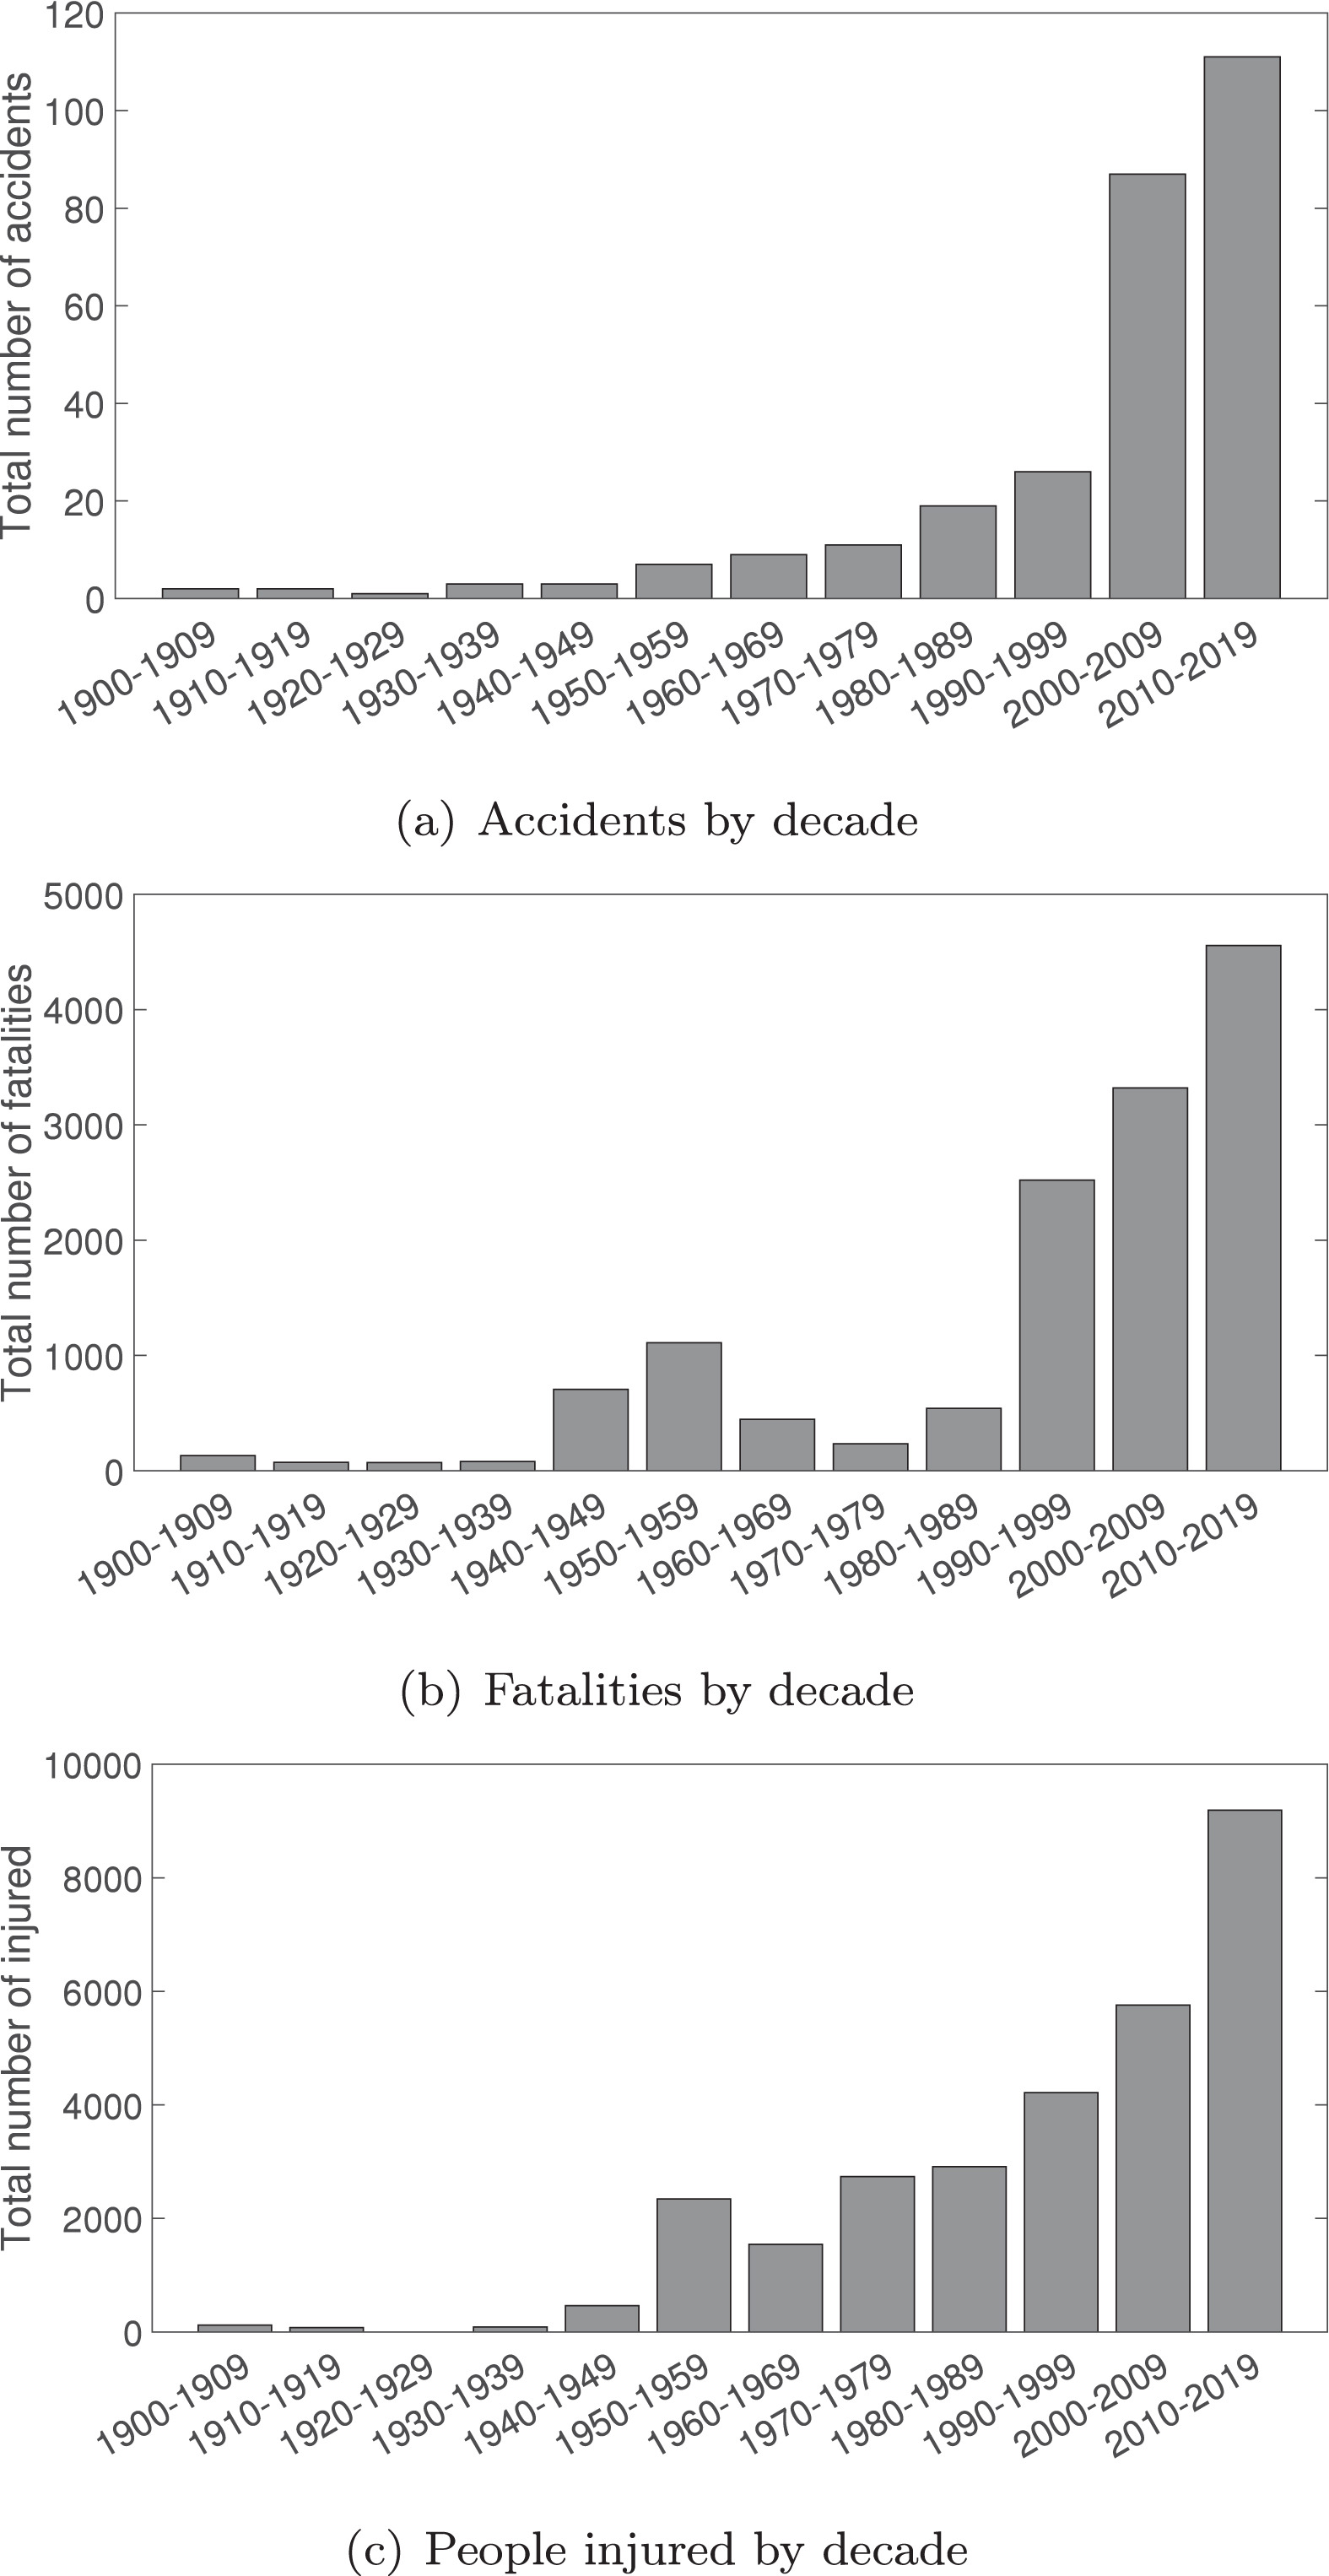
\includegraphics{../images/fatalities.jpg}

}

\caption{\label{fig-fatalities}Fatalities in crowds graph
\autocite[Figure from][]{FELICIANI2023106174}}

\end{figure}

As seen from Figure~\ref{fig-fatalities} accidents, fatalities and
injuries at festivals and concerts worldwide are on the rise, with just
below 5,000 worldwide deaths in the decade of 2010-2019. This can be
attributed to several causes, according to \textcite{inproceedings}:
First of all, an increase in the popularity of outdoor music festivals
resulting in more and larger festivals with large crowds. Also,
high-risk behavior among crowd attendants and the performing artist's
music, behavior, and stage show affects the crowd's safety. Cultural
influence has also played a large part in the safety of outdoor musical
events. This can be behavior such as crowd surfing, moshing, stage
diving and the like. Sudden panic in a crowded place can thus affect the
safety of the crowd.

It is worth mentioning that these figures and descriptions of situations
are from media outlets. As such, it's not the full story. While these
statistics might make it seem that general safety and incidents at
festivals and the like have gotten worse, it is the opposite, It is
generally incredibly safe to attend these events, but using newer
technologies we will attempt to enhance it further.

At the same time, festivals in Denmark and the rest of the world have
had a focus on mitigating the safety risk in large crowds. This can be
seen by the establishment of the
\href{https://eventsafety.dk/historie}{Event Safety Foundation} in 2015.
This is a joint venture between the Skanderborg Festival Group
(Smukfest) and Muskelsvindfonden (Grøn Koncert). This foundation has the
purpose of securing the safety of the crowds at these two large Danish
festivals, as well as many other events in Denmark. They do this through
knowledge sharing, professionals and trained volunteers, courses and
counseling. This is the company that this project will be done in
collaboration with.

To have the best possible outcome for this project, Event Safety invited
us to Grøn Koncert and Smukfest in July and August to see how they work
and gather security video footage of real crowds at festivals to use as
training data. We will also use Event Safety for their practical and
theoretical knowledge of crowd safety to use in the system, user
feedback and user testing.

\hypertarget{problem-statement}{%
\subsection{Problem Statement}\label{problem-statement}}

Can computer vision software and AI techniques be leveraged to improve
crowd overview for security guards, by receiving video feed from large
crowds, and ultimately improve crowd safety?

\newpage{}

\hypertarget{analysis}{%
\section{Analysis}\label{analysis}}

\hypertarget{system-specification}{%
\subsection{System specification}\label{system-specification}}

Using cameras mounted around a hotspot of a crowd or on a stationary
drone, we aim to develop a platform where an AI model receives live
footage from these cameras, uses the model to segment the crowd, and
learns what a dangerous situation might look like. This could be one or
more of the following \autocite{inproceedings}:

\begin{itemize}
\tightlist
\item
  Several people moving into the crowd from a specific direction create
  a dangerous pressure point
\item
  More than a specified amount of people in a marked area resulting in
  unsafe conditions (ie. \textgreater6 people per square meter)
\item
  Omnidirectional or directional movement in the crowd resulting in a
  dangerous situation
\item
  An area in the crowd suddenly being void of people, perhaps hinting at
  a mosh pit or an emergency
\end{itemize}

These are some of the situations this project aims to systematically
detect and alert professionals by providing meaningful feedback.

The system would consist of the following:

\begin{enumerate}
\def\labelenumi{\arabic{enumi}.}
\tightlist
\item
  A backend that receives the data from the cameras developed in either
  Java or Python, with an implementation of a machine learning model to
  handle the video feed according to the bullet list above and exposing
  this data through an API
\item
  A simple frontend or GUI (Graphical User Interface) to display this
  information in a meaningful way. This could be through a heat map, a
  numerical estimate of a risk factor, or other visual output.
\end{enumerate}

\begin{figure}

{\centering 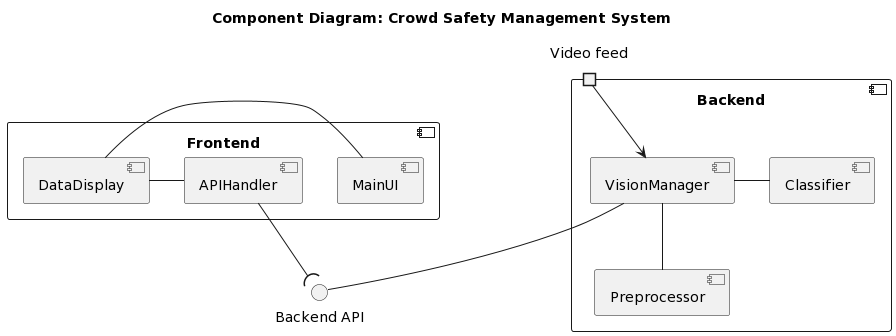
\includegraphics[width=\textwidth,height=0.5\textheight]{../images/component-diagram-1.png}

}

\caption{\label{fig-component-diagram}Component diagram of the system}

\end{figure}

An initial component diagram that maps this described system can be seen
in Figure~\ref{fig-component-diagram}.

\hypertarget{functional-requirements}{%
\subsection{Functional Requirements}\label{functional-requirements}}

\begin{longtable}[]{@{}
  >{\raggedright\arraybackslash}p{(\columnwidth - 4\tabcolsep) * \real{0.0429}}
  >{\raggedright\arraybackslash}p{(\columnwidth - 4\tabcolsep) * \real{0.2000}}
  >{\raggedright\arraybackslash}p{(\columnwidth - 4\tabcolsep) * \real{0.7571}}@{}}
\toprule\noalign{}
\begin{minipage}[b]{\linewidth}\raggedright
\textbf{ID}
\end{minipage} & \begin{minipage}[b]{\linewidth}\raggedright
\textbf{MoSCoW}
\end{minipage} & \begin{minipage}[b]{\linewidth}\raggedright
\textbf{Requirement}
\end{minipage} \\
\midrule\noalign{}
\endhead
\bottomrule\noalign{}
\endlastfoot
1 & M & The system \textbf{must} be able to count the amount of people
in the crowd with a precision of \textless100 MAE \\
& & \\
2 & M & The system \textbf{must} be able to segment the crowd into
virtual sections for further processing \\
& & \\
3 & M & The system \textbf{must} be able to create a heatmap of the
crowd density \\
& & \\
4 & S & The system \textbf{should} be able to calculate the ``real''
density pr. area unit \\
& & \\
5 & S & The system \textbf{should} be able to detect the movement of
crowd sections \\
& & \\
6 & S & The system \textbf{should} be able to correct for camera
distortion, warp and perspective \\
& & \\
7 & S & The system \textbf{should} be able to detect choke points in the
crowd movements \\
& & \\
8 & S & The system \textbf{should} be able to generate a summarizing
report of the concert with statistics of (crowd density, crowd count,
risk factors, choke points, and other) relevant safety indicators after
the event \\
& & \\
9 & C & The system \textbf{could} be able to estimate a numerical risk
factor based on available factors \\
& & \\
10 & C & The system \textbf{could} be able to generate a live, or
delayed, video overlaid user interface \\
& & \\
11 & W & The system \textbf{will not} be able to identify dangerous
situations that might call for cautionary actions such as crowd surge,
mosh pits, falls, blocked exits, etc. \\
& & \\
12 & W & The system \textbf{will not} be able to use data gathered
elsewhere at a concert such as alcohol sales, average crowd age, sound,
artists, etc. to give a more precise crowd profile and thus risk
factor \\
\end{longtable}

\newpage{}

\hypertarget{non-functional-requirements}{%
\subsection{Non-functional
requirements}\label{non-functional-requirements}}

\begin{longtable}[]{@{}
  >{\raggedright\arraybackslash}p{(\columnwidth - 4\tabcolsep) * \real{0.0429}}
  >{\raggedright\arraybackslash}p{(\columnwidth - 4\tabcolsep) * \real{0.2000}}
  >{\raggedright\arraybackslash}p{(\columnwidth - 4\tabcolsep) * \real{0.7571}}@{}}
\toprule\noalign{}
\begin{minipage}[b]{\linewidth}\raggedright
\textbf{ID}
\end{minipage} & \begin{minipage}[b]{\linewidth}\raggedright
\textbf{MoSCoW}
\end{minipage} & \begin{minipage}[b]{\linewidth}\raggedright
\textbf{Requirement}
\end{minipage} \\
\midrule\noalign{}
\endhead
\bottomrule\noalign{}
\endlastfoot
1 & M & The system \textbf{must} protect the privacy of the personal
data \\
& & \\
2 & S & The system \textbf{should} have a user-friendly interface that
is easy to manage for both technical and non-technical users \\
& & \\
3 & S & The system \textbf{should} have adequate documentation /
technical specification for technical users \\
& & \\
4 & S & The system \textbf{should} have adequate user manuals for
non-technical users \\
& & \\
5 & C & The system \textbf{could} have high reliability that is not
based on the visual circumstances and environment (e.g.~sunlight, stage
light, audience flashlights, and other visual effects) or report
confidence based on environment \\
& & \\
6 & C & The system \textbf{could} be scalable to simultaneous
interoperability between multiple cameras \\
& & \\
7 & C & The system \textbf{could} integrate with existing CCTV software
systems at venues \\
\end{longtable}

\newpage{}

\hypertarget{detailed-requirements}{%
\subsection{Detailed Requirements}\label{detailed-requirements}}

\hypertarget{risks}{%
\subsection{Risks}\label{risks}}

More often that not a project will encounter problems that can hinder
the progress or outcome. By being well prepared we are able to mitigate
some of these risks. The following table describes some of the risks we
might encounter in this project.

\begin{longtable}[]{@{}
  >{\raggedright\arraybackslash}p{(\columnwidth - 8\tabcolsep) * \real{0.2000}}
  >{\raggedright\arraybackslash}p{(\columnwidth - 8\tabcolsep) * \real{0.2000}}
  >{\raggedright\arraybackslash}p{(\columnwidth - 8\tabcolsep) * \real{0.2000}}
  >{\raggedright\arraybackslash}p{(\columnwidth - 8\tabcolsep) * \real{0.2000}}
  >{\raggedright\arraybackslash}p{(\columnwidth - 8\tabcolsep) * \real{0.2000}}@{}}
\toprule\noalign{}
\begin{minipage}[b]{\linewidth}\raggedright
\textbf{ID}
\end{minipage} & \begin{minipage}[b]{\linewidth}\raggedright
\textbf{Name}
\end{minipage} & \begin{minipage}[b]{\linewidth}\raggedright
\textbf{Affects}
\end{minipage} & \begin{minipage}[b]{\linewidth}\raggedright
\textbf{Description}
\end{minipage} & \begin{minipage}[b]{\linewidth}\raggedright
\textbf{Mitigation}
\end{minipage} \\
\midrule\noalign{}
\endhead
\bottomrule\noalign{}
\endlastfoot
R01 & Code is lost & Project, product & If the code for some reason is
lost or google colab i suddenly insaccessible & Having backups of our
code on github \\
& & & & \\
R02 & Technology constraints & Product & If the technology previously
used in the project suddenly becomes inadequate for the remaining
requirements defined in the project & Find alternative technologies or
solutions for our requirements before a barrier might be reached.
Discuss with supervisor if alternatives exist. \\
& & & & \\
R03 & Personal Conflicts & Product, project & A project related or
personal conflict between the 2 members of the project having an effect
on either further development or the project as a whole. & Keeping a
friendly and open mindset in the work will take us far. Depending on the
nature of a potential conflict we would either discuss and solve it
outside of work or discuss with our supervisor. \\
& & & & \\
R04 & Unusable data & Project, Product & If the data provided by the
drone or from EventSafety turns out to be unusable due to one or more
factors: Resolution, perspective, Distortion etc. & Making sure that
provided data is on par regarding the requirements of our project. Some
data might be fixed by using mathematics but in general a proper
standard for data is preferred \\
& & & & \\
R05 & Company collaboration ends & Project & If EventSafety or the group
decides to end the collaboration around the project early. & Making sure
that we listen to and adapt to feedback from EventSafety to keep our
good relationship with them \\
\end{longtable}

\hypertarget{risk-assessment}{%
\subsection{Risk assessment}\label{risk-assessment}}

To fully assess the risks described above it is absolutely vital that
the probabality and severity of each individual risk is assessed. This
results in the following formula:

\[
Effect = Probabilty * Severity
\]

The probablity and severity is given each given a score between 1 and 5.
1 being a low probabilty/severity and 5 being a very high
probabilty/severity. The effect is then calculated based on these
numbers.

\begin{longtable}[]{@{}
  >{\raggedright\arraybackslash}p{(\columnwidth - 8\tabcolsep) * \real{0.2000}}
  >{\raggedright\arraybackslash}p{(\columnwidth - 8\tabcolsep) * \real{0.2000}}
  >{\raggedright\arraybackslash}p{(\columnwidth - 8\tabcolsep) * \real{0.2000}}
  >{\raggedright\arraybackslash}p{(\columnwidth - 8\tabcolsep) * \real{0.2000}}
  >{\raggedright\arraybackslash}p{(\columnwidth - 8\tabcolsep) * \real{0.2000}}@{}}
\toprule\noalign{}
\begin{minipage}[b]{\linewidth}\raggedright
\textbf{ID}
\end{minipage} & \begin{minipage}[b]{\linewidth}\raggedright
\textbf{Probablity}
\end{minipage} & \begin{minipage}[b]{\linewidth}\raggedright
\textbf{Severity}
\end{minipage} & \begin{minipage}[b]{\linewidth}\raggedright
\textbf{Effect}
\end{minipage} & \begin{minipage}[b]{\linewidth}\raggedright
\textbf{Notes}
\end{minipage} \\
\midrule\noalign{}
\endhead
\bottomrule\noalign{}
\endlastfoot
R01 & 1 & 3 & 3 & The severity is based on the amount of code lost \\
& & & & \\
R02 & 2 & 2 & 4 & GPU limitations are the primary factor here. However,
we dont see the need for more than what google colab can provide. \\
& & & & \\
R03 & 1 & 1 & 1 & Given the nature of previous work in semester projects
and friendship, this is highly unlikely \\
& & & & \\
R04 & 4 & 3 & 12 & The severity really depends on how bad the data is
and how well we are able to adapt to it \\
& & & & \\
R05 & 1 & 5 & 5 & Severity would depend on when in the process
EventSafety would cancel our collaboration. \\
\end{longtable}

\hypertarget{method-and-theory}{%
\subsection{Method and theory}\label{method-and-theory}}

\hypertarget{convolutional-neural-network-cnn-for-computer-vision}{%
\subsubsection{Convolutional Neural Network (CNN) for Computer
Vision}\label{convolutional-neural-network-cnn-for-computer-vision}}

Convolutional Neural Networks (CNN) are a type of Artificial Neural
Networks (ANN) that are used to ``solve difficult image-driven pattern
recognition tasks.'' \autocite{DBLP:journals/corr/OSheaN15} ANN's
function on an input in the form of a multi-dimensional vectors, which
will be distributed to a number of hidden layers. The hidden layers will
be weighted by evaluating how a stochastic change within itself affects
the final output (backpropagation). Deep learning is an ANN with
multiple hidden layers. ANN's can be either supervised: Being trained on
a set of labeled training data, or unsupervised: Having no labeled
training data, but instead minimizing the result of the cost function.
According to \textcite{DBLP:journals/corr/OSheaN15} and
\textcite{NIPS2010_fe73f687}, supervised learning is usually necessary
for image-focused pattern recognition tasks.

CNN's are similar to ANN's in almost every way, with the only difference
being that CNN's allow to encode image specific features such as edges,
textures, color patterns and shape features. This reduces the complexity
of a traditional ANN trained on image data, where a vector
representation grows in size exponentially depending on the image size.
Reducing the feature vector also reduces the risk of overfitting the
model. This is done through the process of convolution. In the
convolution layer, local regions of the image vector are scanned for
image relevant features. Usually the features are run through a pooling
layer, reducing its computational complexity by sampling and
down-scaling the features. This feature map is then fed to a traditional
ANN, with a given amount of hidden layers.

\hypertarget{solving-scale-variation-with-sasnet}{%
\subsubsection{Solving Scale-Variation with
SASNet}\label{solving-scale-variation-with-sasnet}}

Scale variation is one of the main challenges with crowd counting, since
perspective in the image will lead to different sizes of heads. One
solution to this is proposed by \textcite{sasnet}. SASNet relies on the
fact that heads in a local path share roughly the same scale. It is
currently not a common approach to solve scale variation on a continuous
scale. SASNet solves it discretly but in 5 discrete steps using a
weighted average. This bridges the gap between discrete feature
extraction and continuous feature extraction. This architecture can be
seen in Figure~\ref{fig-sasnet}.

\begin{figure}

{\centering 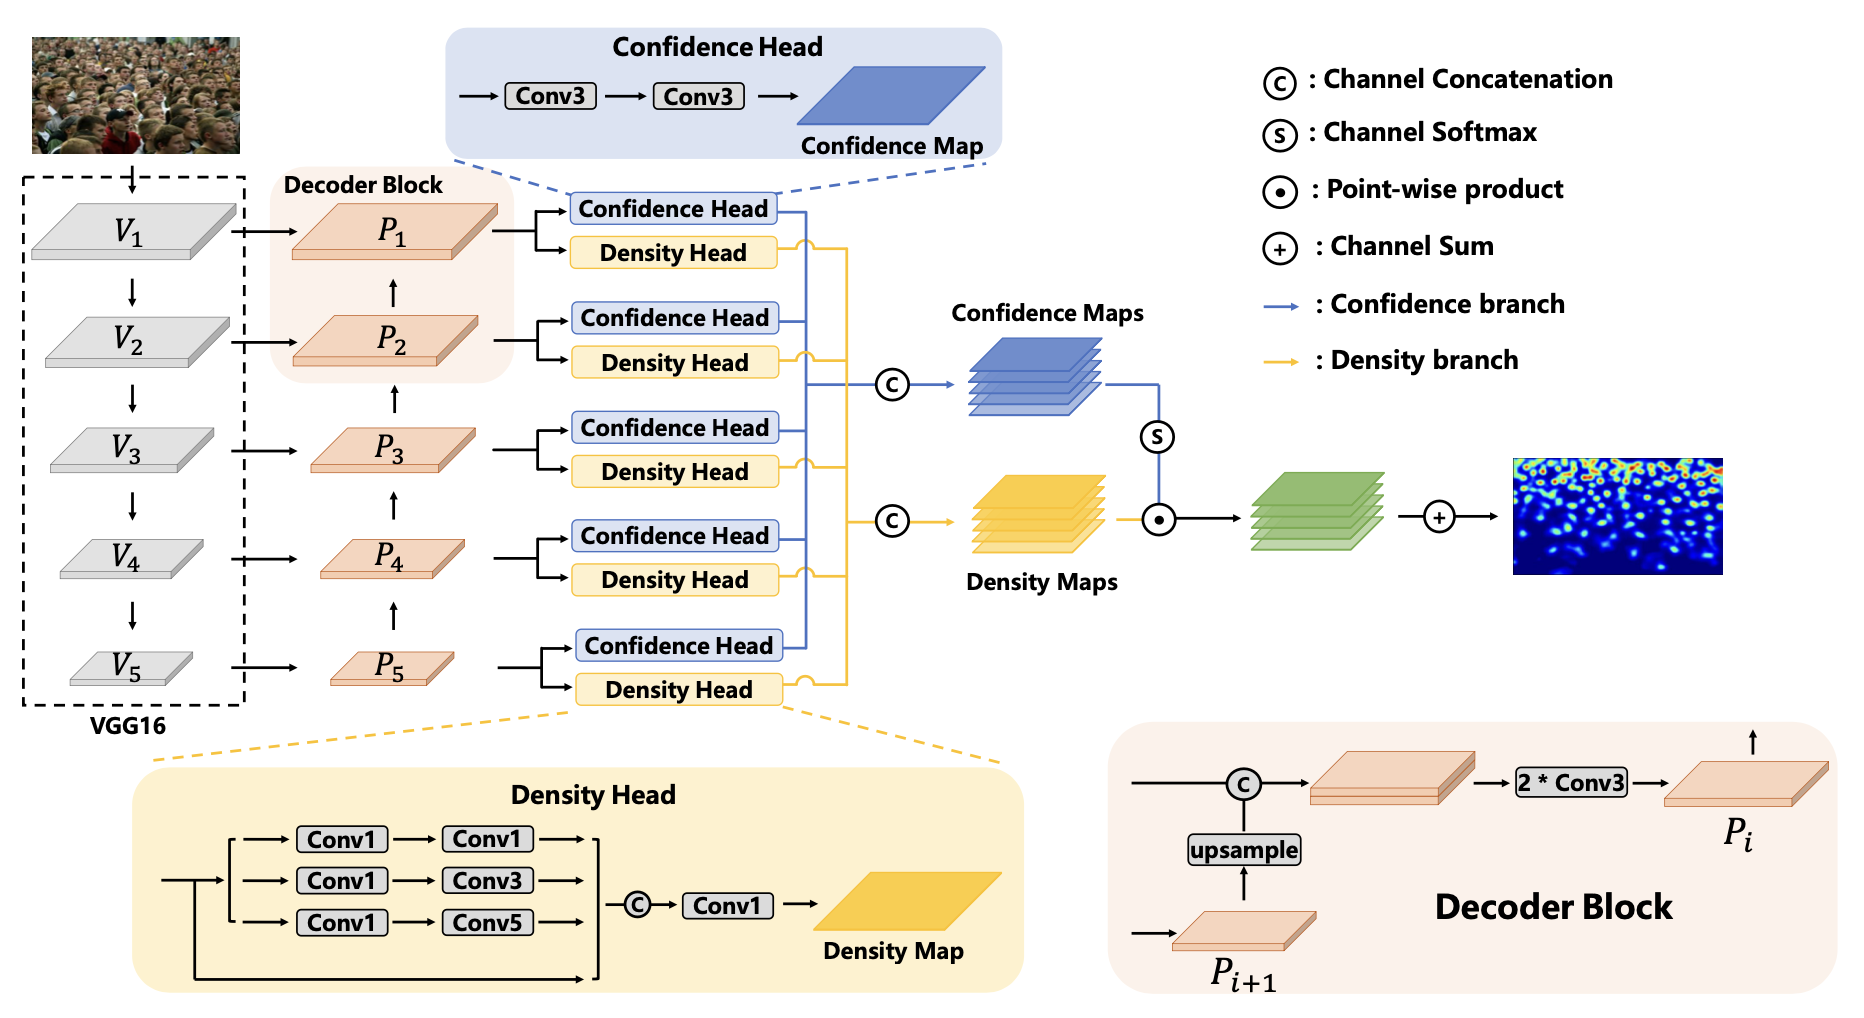
\includegraphics{../images/sasnet-architechture.png}

}

\caption{\label{fig-sasnet}Architecture of the SASNet model
\autocite[Diagram from][]{sasnet}}

\end{figure}

As it can be seen from the diagram, SASNet uses the first 13
convolutional layers from VGG-16 \autocite{simonyan2014very} in the
encoder. SASNet then produces 5 feature levels with 5 levels of
downsampling (\(V_n\)). It produces 5 levels of predictions (\(P_n\)).
This is what is referred to as the ``U-shaped backbone''. These are then
fed to a confidence branch and a density branch that produces a
confidence map and density map for each of the 5 levels. The complete
density map is a product of the sum of the individual density and
confidence branches using a softmax function for the confidence.

\hypertarget{cuda}{%
\subsubsection{CUDA}\label{cuda}}

\newpage{}

\hypertarget{design}{%
\section{Design}\label{design}}

\hypertarget{about-crowd-counting}{%
\subsection{About Crowd Counting}\label{about-crowd-counting}}

Crowd counting is a field of computer vision research that has developed
quickly in recent years. It is a technique that aims to count the
instances of any object in an image, no matter the context, density or
type of object. \autocite{sasnet} This differentiates it from object
detection which is usually trained on one specific type of object by
extracting certain visual features. The benefits from using crowd
counting rather than object detection is:

\begin{itemize}
\item
  Crowd counting is less intensive on computing resources.
\item
  Crowd counting performs better in crowded scenes with varying scales
  of objects and overlapping objects.
\item
  Crowd counting is more robust in environments with changes in light,
  without the need of specific training data.
\item
  Crowd counting is not as exposed to the risk of over fitting the
  model. \autocite{li2021approaches}
\item
  Crowd counting does not single out individuals, but looks at the crowd
  holistically \autocite{chan2008}
\end{itemize}

For these reasons crowd counting is a method that can be used for many
domains including traffic and parking analysis, pedestrian crowds, corn
and crop counting, and much more. This project will use crowd counting
methods to analyse, count and estimate density of concert crowds.

\autocite{li2021approaches} says the current leading approach to crowd
counting is the use of a CNN. This paper, contrary to our definiton of
crowd counting, includes object detection as a method of crowd counting.
It also includes regression based methods and, of course, CNN's. The
main challenge with CNN's for crowd counting is to differentiate between
the large scale variations in the countable human heads.
\autocite{li2021approaches} discuss several categories of approaches for
CNN based models to solve the scale variation problems, one of which is
multi-scale fusion. This approach is the category that this paper
proposes for further research, as it shows promising results in the
balance between performance and accuracy.

For the reasons outlined here from
\textcite{DBLP:journals/corr/OSheaN15} and \textcite{li2021approaches},
this project will focus on the use of CNN based models for crowd
counting.

One of the useful datasets for crowd counting, ``Shanghaitech'' comes
from the paper \textcite{Zhang_2016_CVPR}. In this paper there are
defined two datasets, ``part a'' and ``part b''. For the purposes of the
CSMS test data, ``Shanghaitech Part A'' is a more representative dataset
to use, since it contains more densely populated crowds from a birds eye
view. The dataset is labeled with one dot representing roughly the
middle of a person's head. This is the approach outlined in one of the
founding papers of crowd counting \textcite{NIPS2010_fe73f687}. In
\textcite{NIPS2010_fe73f687}, it is explained how their approach to
crowd counting, which has become the primary method in the field, is to
create a density function \(F\) as a function of the pixels in an image
\(I\). This density function is analoguous to the physical idea of
density, however not a direct representation of the same concept, as
physical density is based on physical area. Integrating \(F\) over the
entire image \(I\) will return the number of people in \(I\).
\autocite{NIPS2010_fe73f687} Each object in the image I should be
represented by a normalized 2D Gaussian kernel with the mean at the
person's head. One disadvantage with this approach, is that the kernel
for objects close to the edge of the image will not be counted as a
whole object when summed. It is not assumed that this will pose a
significant source of error for the purpose of the CSMS.

\hypertarget{regarding-sam-model-for-crowd-counting}{%
\subsection{Regarding SAM model for Crowd
Counting:}\label{regarding-sam-model-for-crowd-counting}}

One of the original ideas for solving this problem was to use Meta's SAM
model. During the preliminary research sessions, it was discovered that
SAM was not adequate in counting people but better suited for object
detection. The following citation from \textcite{ma2023sam} highlights
the problems well:

``Although the Segment Anything model (SAM) has shown impressive
performance in many scenarios, it currently lags behind state-of-the-art
few-shot counting methods, especially for small and congested objects.
We believe that this is due to two main reasons. Firstly, SAM tends to
segment congested objects of the same category with a single mask.
Secondly, SAM is trained with masks that lack semantic class
annotations, which could hinder its ability to differentiate between
different objects. Nevertheless, further exploration of adapting SAM to
the object counting task is still worth studying.'' \autocite{ma2023sam}

\hypertarget{the-choice-of-sasnet}{%
\subsection{The choice of SASNet}\label{the-choice-of-sasnet}}

The choice of using SASNet was based on three different factors:

\begin{enumerate}
\def\labelenumi{\arabic{enumi}.}
\item
  SASNets fits our need to solve the problem of scale variation in the
  video material. It was not possible to obtain video material from an
  approximate orthographic perspective. However, future endeavors for
  this project might include cameras like those from one of our
  collaborators \href{https://www.phaseone.com/}{PhaseOne} who produces
  approximate orthographic perspectives using high pixel density cameras
  from high altitudes. SASNet, however, fulfills the requirement to
  produce relatively high accuracy on an image with perspective for now.
\item
  SASNet has some of the lowest absolute errors on the ShanghaiTech
  testing data, according to \textcite{gjy3035_awesome_crowd_counting}
  which compares at least 45 different crowd counting models and
  methods.
\item
  SASNet is open source and licensed under the permissive Apache 2.0
  license, which allows us to use it legally and for free in our
  project. SASNet also publishes the pretrained model weights (trained
  on ShanghaiTech A and B), which means we can save many compute- and
  time resources on training the model ourselves.
\end{enumerate}

Finally, SASNet publishes the model weights from the training on either
ShanghaiTech part A or part B. For this project, it is deemed more
useful to use the images from part A. While the labeled dataset is
smaller in part A than part B, it more closely represents the data
(i.e.~amount of people, density and perspectives) that will be used in
this project.

\hypertarget{activity-diagram}{%
\subsection{Activity diagram}\label{activity-diagram}}

Figure~\ref{fig-activity-diagram} illustrates the flow of the program
through an activity diagram. The diagram was created to obtain a deeper
understanding of the general flow and processes the program goes through
during its runtime. The diagram is split into 2 ``swimlanes'', one lane
for our CSMS system and one lane for the implementation of the SASNet
model. In broad terms, this can also be specified as a CPU and a GPU
lane where our CSMS system handles CPU processing and SASNet focuses on
GPU processing.

As depicted in the diagram, section of the activities are divided into
partitions to visualise a rough partioning into classes and for better
readability throughout the diagram. The input is specified as the path
to the pretrained model and the path to the video for it to run on.

Below is a short runthrough of the different partitions. A more indepth
description can be found in the implemetation section

\begin{enumerate}
\def\labelenumi{\arabic{enumi}.}
\tightlist
\item
  System Initialization and Input Validation
\end{enumerate}

The CSMS is initialized and the inputs for the model and video path are
validated

\begin{enumerate}
\def\labelenumi{\arabic{enumi}.}
\setcounter{enumi}{1}
\tightlist
\item
  SASNet Model Setup and Construction
\end{enumerate}

The SASNet model is loaded together with VGG16 model which it is based
on. This sets the foundation for subsequent image processing.

\begin{enumerate}
\def\labelenumi{\arabic{enumi}.}
\setcounter{enumi}{2}
\tightlist
\item
  Pre-Processing of Input Data
\end{enumerate}

Preprocessing involves creating a dataset from the video in pyTorch and
in turn creating a dataloader from this dataset.

\begin{enumerate}
\def\labelenumi{\arabic{enumi}.}
\setcounter{enumi}{3}
\tightlist
\item
  Image processing Loop
\end{enumerate}

The images in the dataloader are iterated through and forwarded to the
SASNet model until the dataloader is empty. Each image processed through
the different layers to prepare them for post-processing

\begin{enumerate}
\def\labelenumi{\arabic{enumi}.}
\setcounter{enumi}{4}
\tightlist
\item
  Post-Processing \& Result Generation
\end{enumerate}

Following the image processing, the CSMS takes over again. Here density
information is computed, perspective warping is applied to in turn
generate the correct heatmap for further analysis.

\begin{enumerate}
\def\labelenumi{\arabic{enumi}.}
\setcounter{enumi}{5}
\tightlist
\item
  Output Generation \& Reporting
\end{enumerate}

All of the crowd counting data is saved to a CSV filed and the images
are stitched together to form a timelapse and a report, summarizing the
observations.

\begin{figure}

{\centering 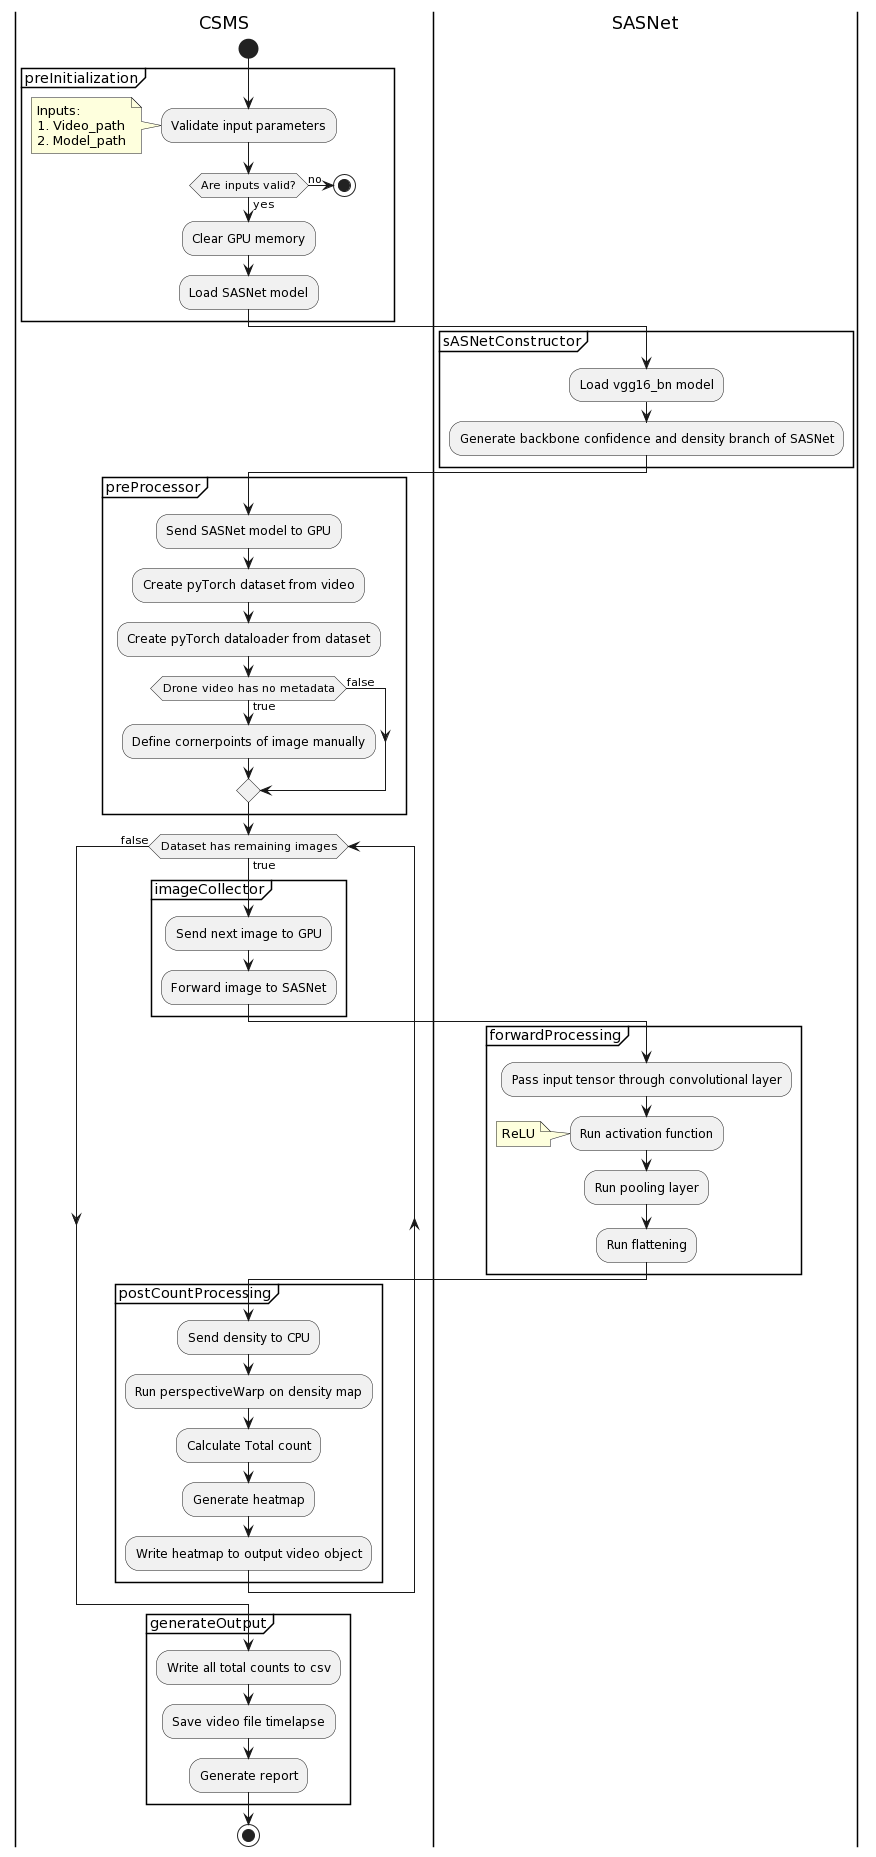
\includegraphics{../images/activity-diagram-1.png}

}

\caption{\label{fig-activity-diagram}Activity diagram depicting flow in
the solution}

\end{figure}

\newpage{}

\hypertarget{implementation}{%
\section{Implementation}\label{implementation}}

\hypertarget{data-collection-and-preparation}{%
\subsection{Data Collection and
Preparation}\label{data-collection-and-preparation}}

To implement this project it was necessary to gather useful evaluation
data. For the purposes of this project, that is video security footage
and drone footage. Our collaborative partner EventSafety was very
helpful in letting us gather this data at their 2 festivals,
``Smukfest'' and ``Grøn''. This was done 1-2 months before the project
started since this is when the festivals were held. This means that we
gathered the data before completing the research on crowd counting and
computer vision. It did pose a challenge to collect the data before
knowing exactly what type of data was needed. For these reasons, we
collected many types of data, including:

\begin{enumerate}
\def\labelenumi{\arabic{enumi}.}
\item
  Drone footage from ``Grøn'' at an altitude of 25-50 meters from the
  entrance
\item
  Drone footage from ``Grøn'' at an altitude of 25-50 meters of the
  concerts and end of concerts
\item
  GoPro footage from ``Grøn'' at an altitude of 2-5 meters from the
  entrance
\item
  Security camera footage from ``Smukfest at an altitude of
  approximately 10-15 meters from the center of the stage.
\item
  Security camera footage from ``Smukfest'' at various heights from bars
  and paths
\end{enumerate}

What turned out to be most useful was option no. 2, drone footage from
``Grøn'' at an altitude of 25-50 meters of the concerts. Having a
perspective from a higher altitude means that more people are clearly
visible and also minimizes distortion when warping for perspective
correction. Having an even higher resolution from a higher altitude
could also increase the accuracy of the predictions. The resolution of
the drone footage was 1080p. Having a higher resolution could limit the
video compression artifacts. The camera options were discussed with our
secondary partner PhaseOne. They have experience with
ultra-high-resolution top-down drone footage. This could be an option
for future endeavors, which will be discussed in
Section~\ref{sec-perspective} section of this report.

While we, with the help of a certified drone pilot, collected the
footage from ``Grøn'' ourselves, the security footage from ``Smukfest''
was collected by EventSafety. For this, we created a technical
specification with our requirements for the footage at the time. This
can be read in \textbf{?@fig-camera-specs} in
Section~\ref{sec-appendices}.

\hypertarget{environment}{%
\subsection{Environment}\label{environment}}

Setting up an environment for machine learning in Python can pose a bit
of a challenge. Is a requirement to have access to a NVIDIA GPU to take
advantage of the CUDA toolkit in PyTorch. This opens up GPU acceleration
which enables a large performance boost rather than running the CNN
models on the CPU. Furthermore, the SASNet open source projects were
built for Python 3.6.8 and PyTorch \textgreater= 1.5.0
\textcite{sasnet}.

\hypertarget{google-colab}{%
\subsubsection{Google Colab}\label{google-colab}}

Because of these strict software and hardware requirements, we decided
to use the virtual environment in
\href{https://research.google.com/colaboratory/faq.html}{Google Colab}.
Google Colab provides a preconfigured Python environment with (free but
not unlimited) access to a NVIDIA GPU. Doing this project in the cloud
removes the software and hardware limitations on both the users and
developers of the project. However, Google Colab has some feature
limitations such as it being disallowed to use it for the purpose of
hosting web services. Google Drive can then be volume mounted inside the
virtual environment making it possible to use and make persisted files.

The Python version in Google Colab is downgraded to match the version
needed for SASNet and both PyTorch and the required PIP packages are
installed.

\hypertarget{ucloud}{%
\subsubsection{UCloud}\label{ucloud}}

University of Southern Denmark provides a cloud computing service for
faculty members through
\href{https://escience.sdu.dk/index.php/national-hpc-systems/}{eScience}.
Our supervisor applied through this site for a cloud computing resource
with 100 GPU hours.

\hypertarget{sasnet-model-adaption}{%
\subsection{SASNet Model Adaption}\label{sasnet-model-adaption}}

The SASNet model is loaded using pre-trained weights and biases for the
underlying vgg16\_bn model trained on ImageNet. This allows SASNet to
more efficiently identify image features with low memory usage.
Furthermore, the SASNet weights and bias fine-tunings are loaded into
the model which has been trained on the Shanghai Tech Part A dataset. A
block size of 32 is being used here.

\begin{Shaded}
\begin{Highlighting}[]
\KeywordTok{class}\NormalTok{ Args:}
\NormalTok{  model\_path }\OperatorTok{=} \StringTok{"\textless{}path{-}to{-}model{-}dir\textgreater{}/SHHA.pth"}
\NormalTok{  video\_path }\OperatorTok{=} \StringTok{"\textless{}path{-}to{-}input{-}video{-}dir\textgreater{}/DJI\_0461\_trimmed.MP4"}
\NormalTok{  block\_size }\OperatorTok{=} \DecValTok{32}
\NormalTok{  use\_pretrained }\OperatorTok{=} \VariableTok{True}

\NormalTok{model }\OperatorTok{=}\NormalTok{ SASNet(args.use\_pretrained, args).cuda()}
\NormalTok{model.load\_state\_dict(torch.load(args.model\_path))}
\end{Highlighting}
\end{Shaded}

A quick note on block size. Block size is important because when loading
data into a CNN model (or any model for that matter) minimal data
variance is key. For this reason, a block size is added to make sure
that each data input is the same length, see example below:

\begin{Shaded}
\begin{Highlighting}[]
\NormalTok{Hello SDU}
\NormalTok{This }\KeywordTok{is}\NormalTok{ a cool project}
\end{Highlighting}
\end{Shaded}

say our input block size was set to 2, this would make sure that each of
those lines was truncated to a set length, in this case, a length of 10:

\begin{Shaded}
\begin{Highlighting}[]
\NormalTok{Hello SDU }\DecValTok{0} \DecValTok{0}     \DecValTok{0}       \DecValTok{0} \DecValTok{0} \DecValTok{0} \DecValTok{0} \DecValTok{0} 
\NormalTok{This  }\KeywordTok{is}\NormalTok{  a cool  project }\DecValTok{0} \DecValTok{0} \DecValTok{0} \DecValTok{0} \DecValTok{0}
\end{Highlighting}
\end{Shaded}

\hypertarget{integeration}{%
\subsection{Integeration}\label{integeration}}

\hypertarget{optimization-and-performance}{%
\subsection{Optimization and
Performance}\label{optimization-and-performance}}

For two main reasons, it is necessary to limit the compute resource
usage:

\begin{enumerate}
\def\labelenumi{\arabic{enumi}.}
\item
  This project is using free and limited GPU and compute resources.
  Computer vision and CNN's can be very GPU intensive, so it is in the
  project's to limit the GPU memory consumption as this was found to be
  the largest resource bottle neck.
\item
  For the CSMS to be scalable to (near) real-time evaluation
  performance, it makes sense to limit the use of computing power as
  much as possible.
\end{enumerate}

According to \textcite{pytorch},
\href{https://pytorch.org/docs/stable/generated/torch.no_grad.html}{disabling
gradient calculation} is useful for lowering memory usage when using a
model for inference. This fits the use case and greatly reduced the
memory usage. This was done using the following way:

\begin{Shaded}
\begin{Highlighting}[]
\NormalTok{img }\OperatorTok{=}\NormalTok{ img.cuda()}
\ControlFlowTok{with}\NormalTok{ torch.no\_grad():}
\NormalTok{  model.}\BuiltInTok{eval}\NormalTok{()}
\NormalTok{  pred\_map }\OperatorTok{=}\NormalTok{ model(img)}
\NormalTok{pred\_map }\OperatorTok{=}\NormalTok{ pred\_map.data.cpu().numpy()}
\end{Highlighting}
\end{Shaded}

Here the image tensor is first sent to the NVIDIA GPU using img.cuda().
Gradient calculations are then disabled for the inference, and the model
is set to eval mode. These two reduce the GPU memory usage. Finally,
after the inference is run and the predicition\_map is calculated, the
tensor data is sent to the cpu and the tensor is converted to a numpy
matrix (an image). This way limits the time that the tensor spends in
the GPU greatly, as well as reducing the memory usage.

\hypertarget{error-handling-security-and-privacy}{%
\subsection{Error Handling, Security and
Privacy}\label{error-handling-security-and-privacy}}

\hypertarget{error-handling}{%
\subsubsection{Error Handling}\label{error-handling}}

One of the major error-handling implementations made is checking if the
data uploaded to the model is present and valid. If either of these
checks fail, the code is not run and the program shuts down.

\hypertarget{security}{%
\subsubsection{Security}\label{security}}

\hypertarget{privacy}{%
\subsubsection{Privacy}\label{privacy}}

Being citizens of and using the data of people from an EU country means
that we have to abide by the rules of GDPR. This means that security and
privacy around the data that we have acquired are crucial. Practically,
this means that we have a responsibility to make sure that we only
upload the images and videos we need to run the model on when they need
to be there and remove them when not needed. In a perfect world, we
would run our program locally to limit the uploading and removal of
sensitive data.

\hypertarget{facial-recognition-vs.-crowd-counting}{%
\subsubsection{Facial recognition vs.~Crowd
Counting}\label{facial-recognition-vs.-crowd-counting}}

When reading about this project, one might assume that privacy around
facial recognition would be an issue. However, as this is related to
heatmaps and crowd density instead of direct recognition of people, the
identity of people in our footage is not a major concern and thus was
not featured in our risk management section. The CSMS does not track
individuals through time, which could be a privacy concern.

\newpage{}

\hypertarget{validation-and-verification}{%
\section{Validation and
Verification}\label{validation-and-verification}}

Since this project is a proof of concept, unit tests and integration
tests are not as favored as user tests and similar. Testing of this
system relies on making sure that it is useful and understandable to
those who need it. To accomplish these tests, we decided to get the
opinions of some EventSafety security personnel about our project and
their thoughts.

\hypertarget{eventsafety-presentation}{%
\subsection{EventSafety presentation}\label{eventsafety-presentation}}

Based on the analysis, design and development of the crowd management
system we were invited to present our project to more people from
EventSafety. Based on this invitation it was decided to research how a
proper focus group is structured and managed properly.

\hypertarget{focus-group}{%
\subsubsection{Focus group}\label{focus-group}}

``As a summative evaluation, focus groups can be used to assess the
acceptance of a new campaign or gauge customer satisfaction levels''
\textcite{designers_research_manual} Based on research from
\textcite{designers_research_manual} we arrived at the following
conclusion for our research group:

\begin{itemize}
\tightlist
\item
  A group of 6-9 people is the preferred group size
\item
  A group of similarly experienced people is needed to encourage a
  proper discussion
\item
  If possible, have more groups with different people
\end{itemize}

For the presentation, a group of 10 employees from Eventsafety attended
the presentation with questions and feedback for us along the way. The
employees all had major experience with crowd management and event
planning. Most of them had heard of our project beforehand but had no
further technical insight.

\hypertarget{questionaire}{%
\subsubsection{Questionaire}\label{questionaire}}

Following the focus group, a questionnaire is conducted to gain further
insight. Normally, a questionnaire is used to gather information from a
large group. For our presentation, we still felt a questionnaire was
relevant to gather solid data for a project report and validation of the
project as a whole.

The questionnaire was conducted using Mentimeter and consisted of
scales, open-ended questions and rankings. This section will highlight
some of the answers the attendees provided. All the questions and their
results (in danish) are found in Section~\ref{sec-appendices}.

\textbf{Question 2} 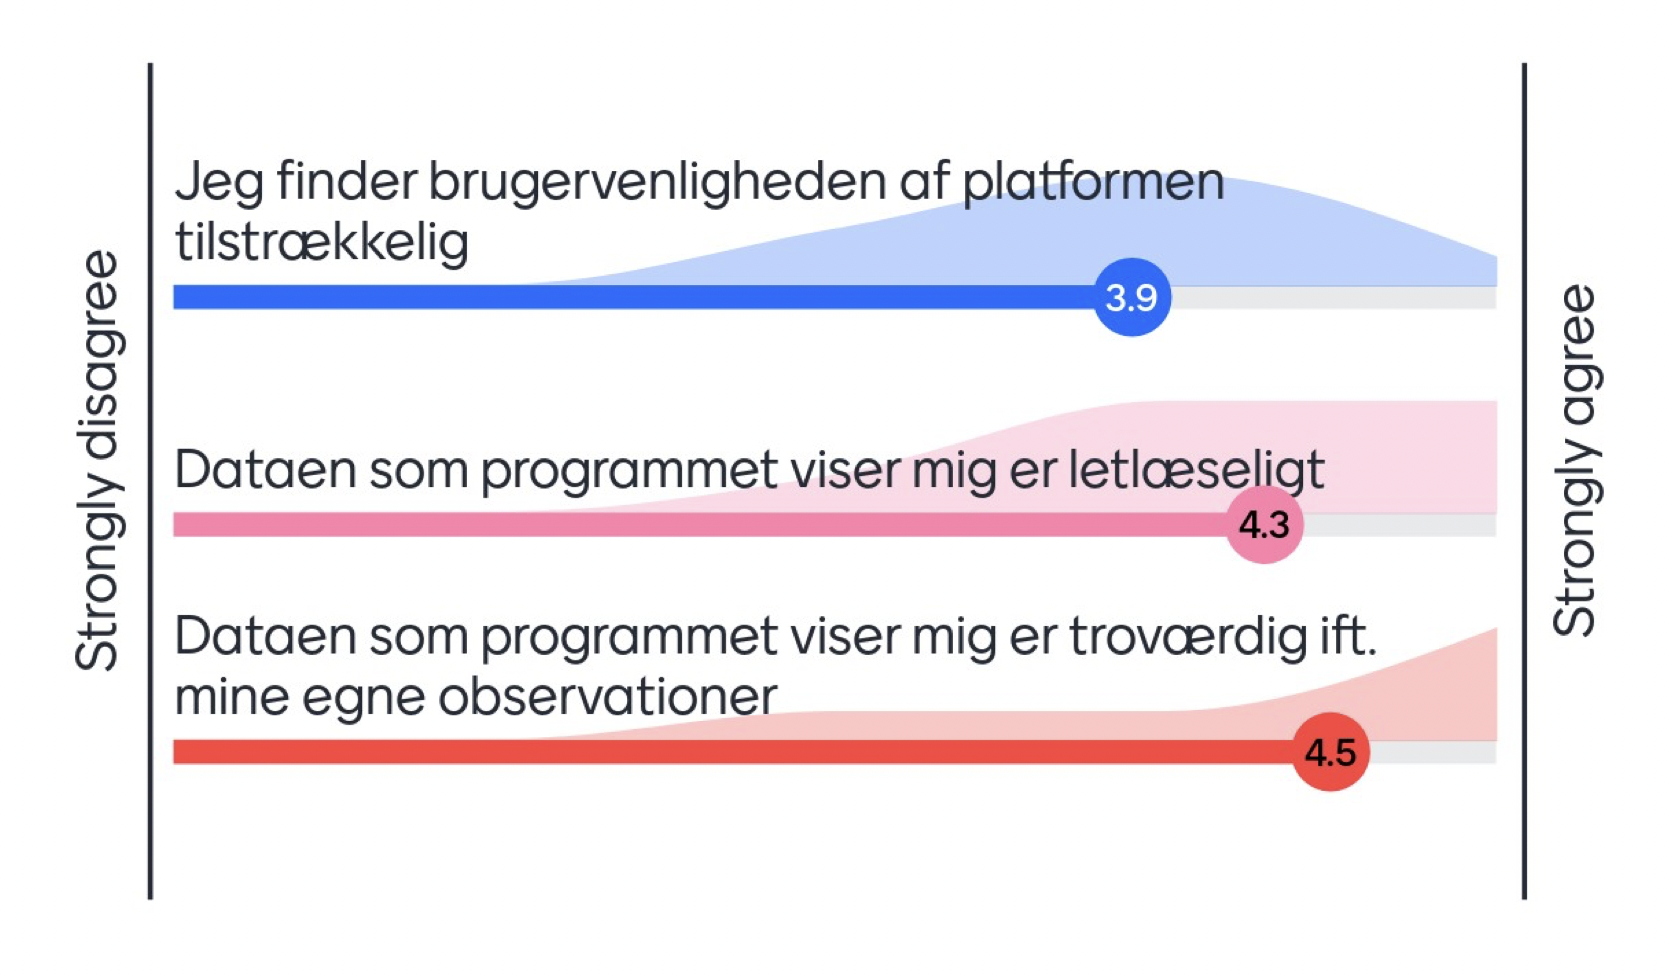
\includegraphics{../images/Evaluation_question2.png}

Question 2 had the attendees evaluate 3 statements on a scale of 1 to 5
and ``strongly disagree'' to ``strongly agree''. 1 being disagree and 5
being agree. The 3 statements were as follows: 1. I find the usability
of the platform adequate 2. The data the program visualizes is easy to
read and understand 3. The data the program provides is credible
compared to my own observations

The first statement was evaluated to a score of 3.9, showing that while
the platform in general seems intuitive and fulfills non-functional
requirement \#2, there is room for visual improvements.

Statement 2 further validates the implementation of non-functional
requirement 2\# with a score of 4.3

Statement 3 shows that the professional observations from our attendees
align with the output of our program, showing that functional
requirement \#1 is fulfilled. An attendee also mentioned that the
heatmap provided by the program gives more value than a precise count of
individuals in a crowd. This comment was unfortunately not documented.

\textbf{Question 3} 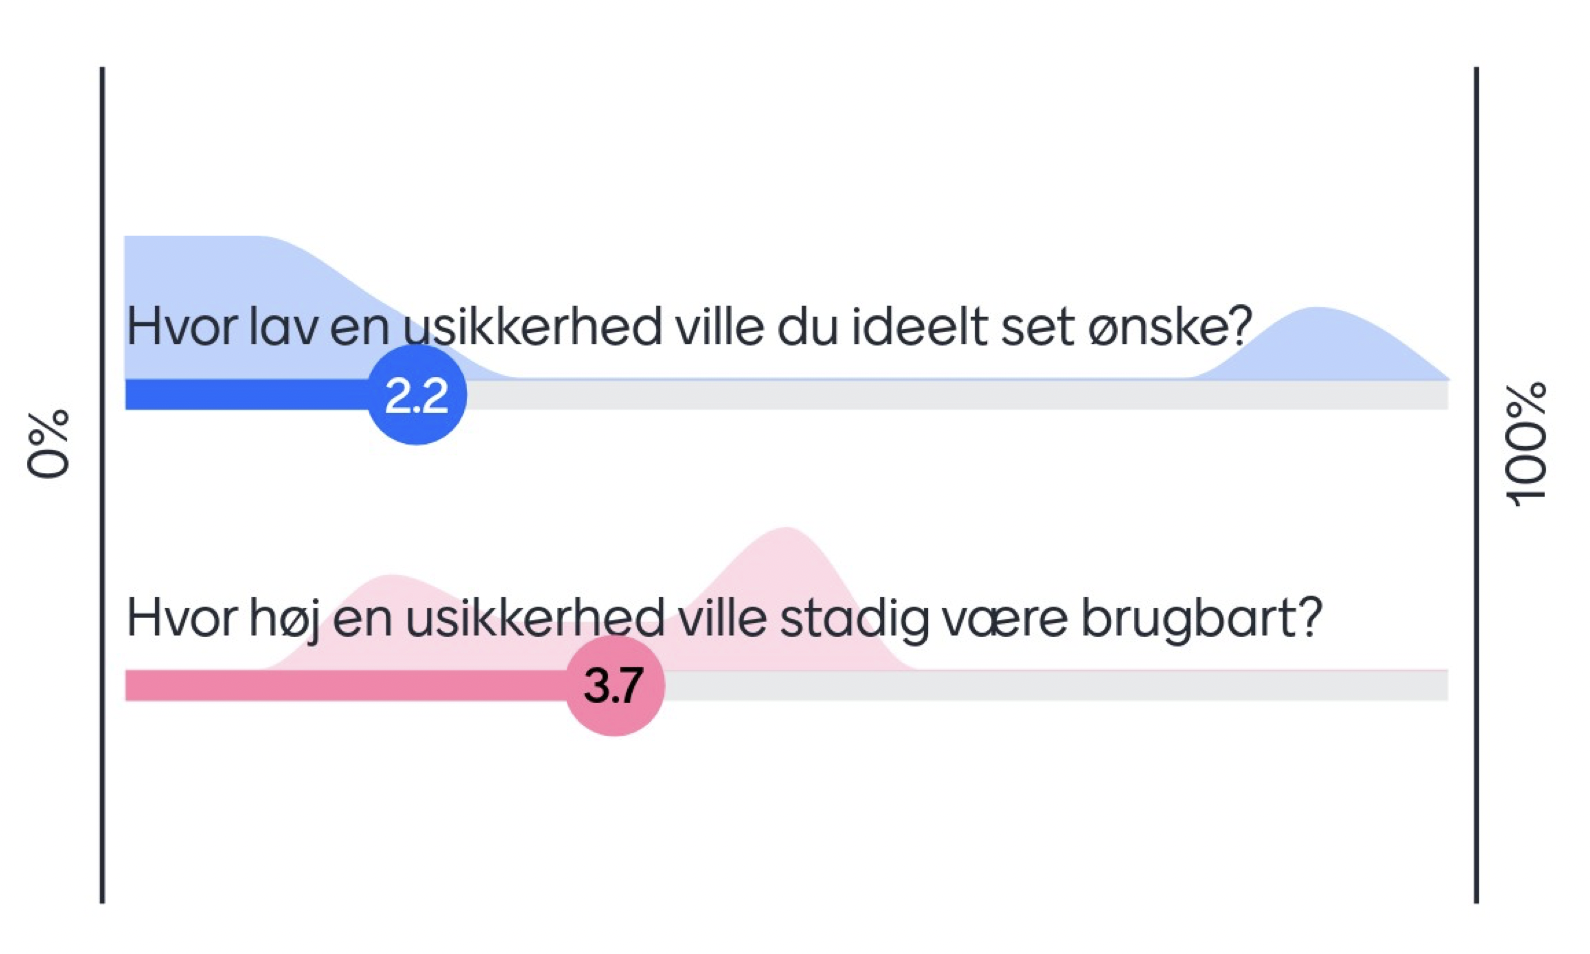
\includegraphics{../images/Evaluation_question3.png}

Question 3 had the attendees evaluate 2 statements from 0 to 100\% based
on their preferred uncertainty of the data provided.

\begin{enumerate}
\def\labelenumi{\arabic{enumi}.}
\tightlist
\item
  What percentage of uncertainty would you prefer?
\item
  How high of an uncertainty would you be willing to accept?
\end{enumerate}

Question 1

\hypertarget{runtime-and-gpu-usage}{%
\subsection{Runtime and GPU usage}\label{runtime-and-gpu-usage}}

While GPU usage is something already discussed in implementation,
runtime and the optimization of this is still crucial to test. While we
originally wanted this project to be able to run in real-time, we
quickly realized that this was close to impossible with our current
setup and implementation. When running the model on a video, we
originally ran it on a 3-minute clip with an image every 10 seconds
being processed. This resulted in a 6-second video and a runtime of the
program of around 15 minutes. Not great, not terrible. In the future, if
we want to run this live, additional resources are required. More about
this in Section~\ref{sec-perspective}

\newpage{}

\hypertarget{discussion}{%
\section{Discussion}\label{discussion}}

TODO: Add section on possibilities with PhaseOne

\newpage{}

\hypertarget{conclusion}{%
\section{Conclusion}\label{conclusion}}

\newpage{}

\hypertarget{sec-perspective}{%
\section{Perspective}\label{sec-perspective}}

\newpage{}

\hypertarget{references}{%
\section{References}\label{references}}

\hypertarget{sec-appendices}{%
\section{Appendices}\label{sec-appendices}}

\textless\textless\textless\textless\textless\textless\textless{} HEAD
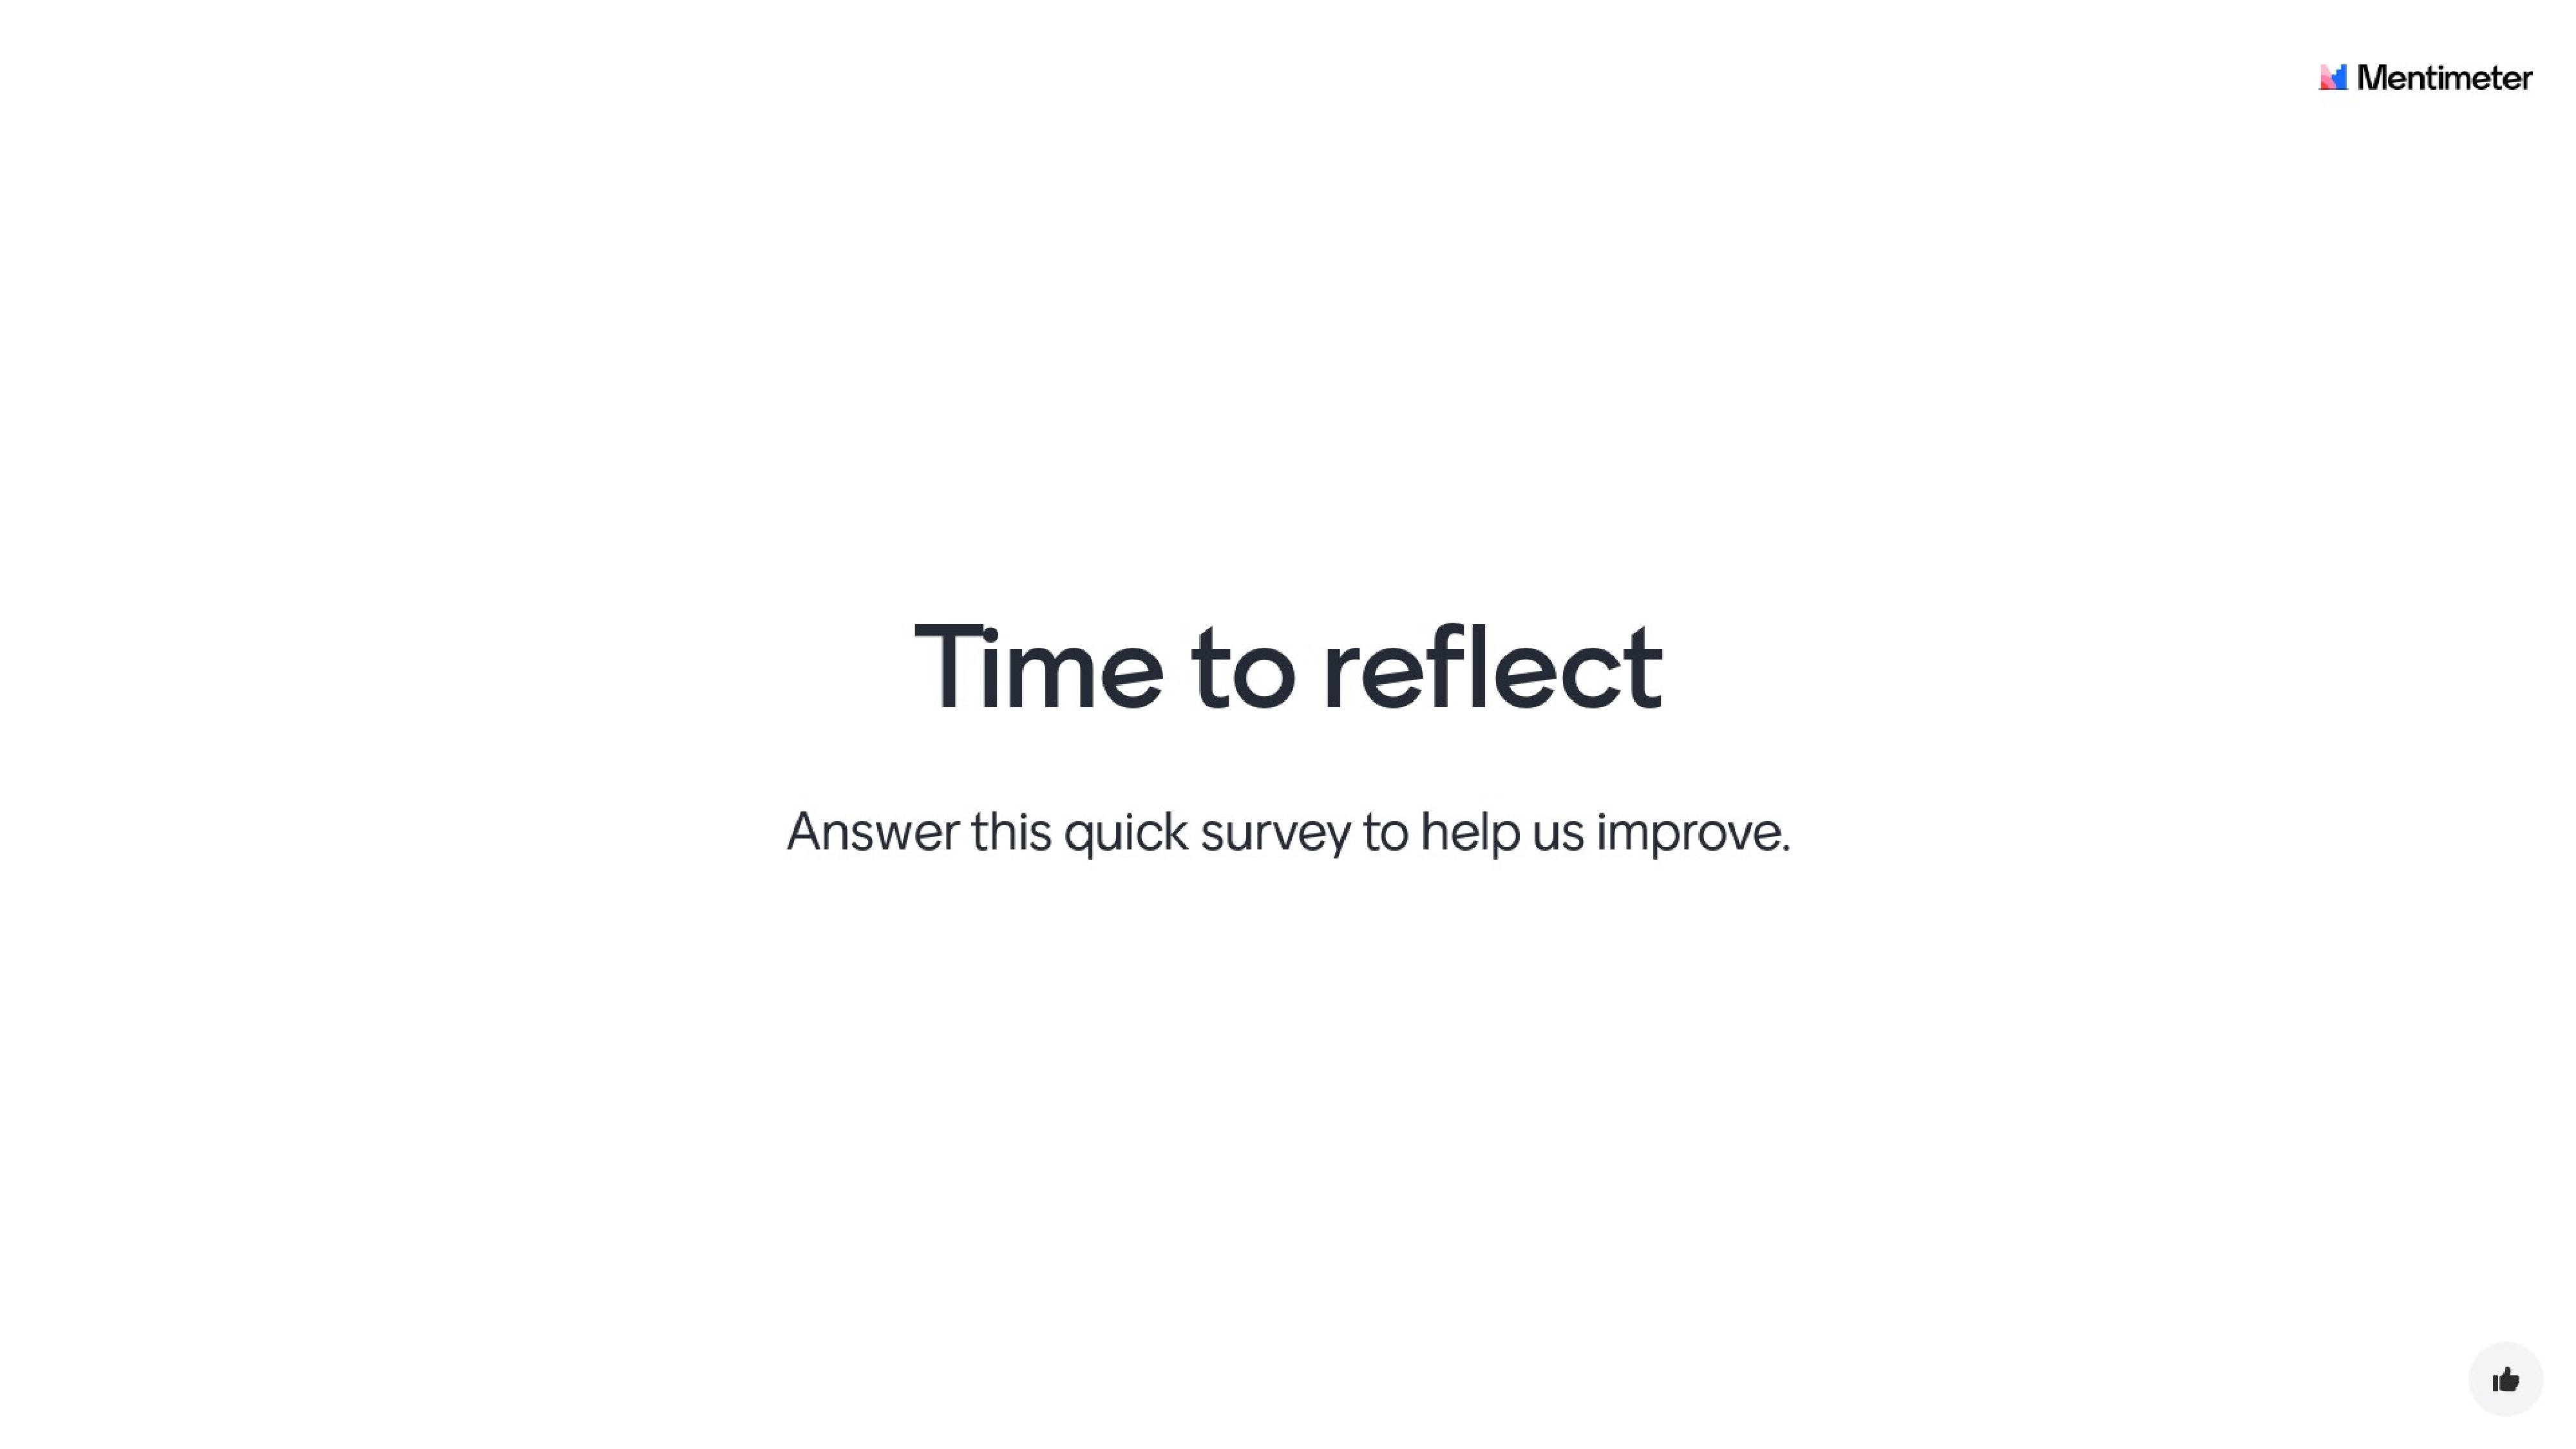
\includegraphics{../appendices/MentimeterPresentation.pdf}(\#fig-presentation-results)
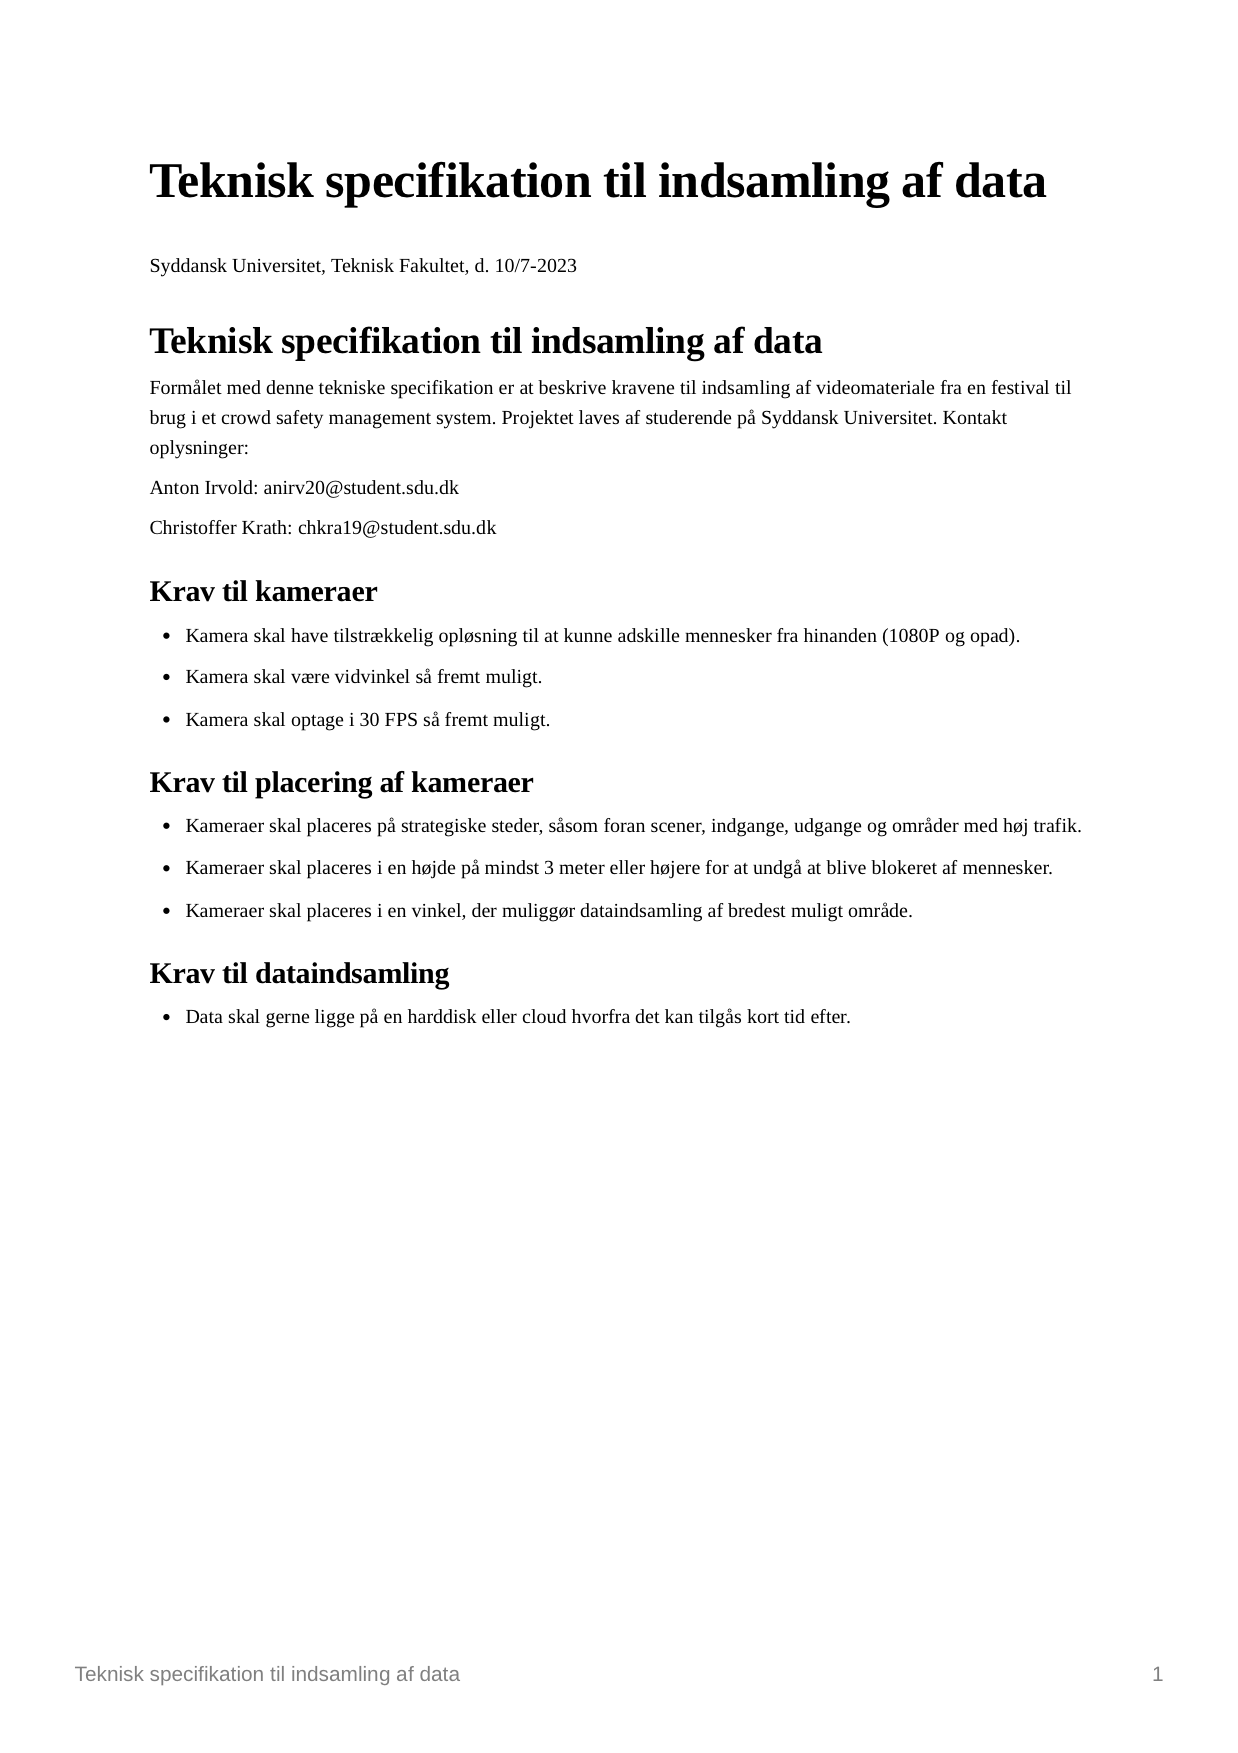
\includegraphics[width=1\textwidth,height=1\textheight]{../appendices/teknisk-specifikation.png}
======= \#\# Technical specifications for camera
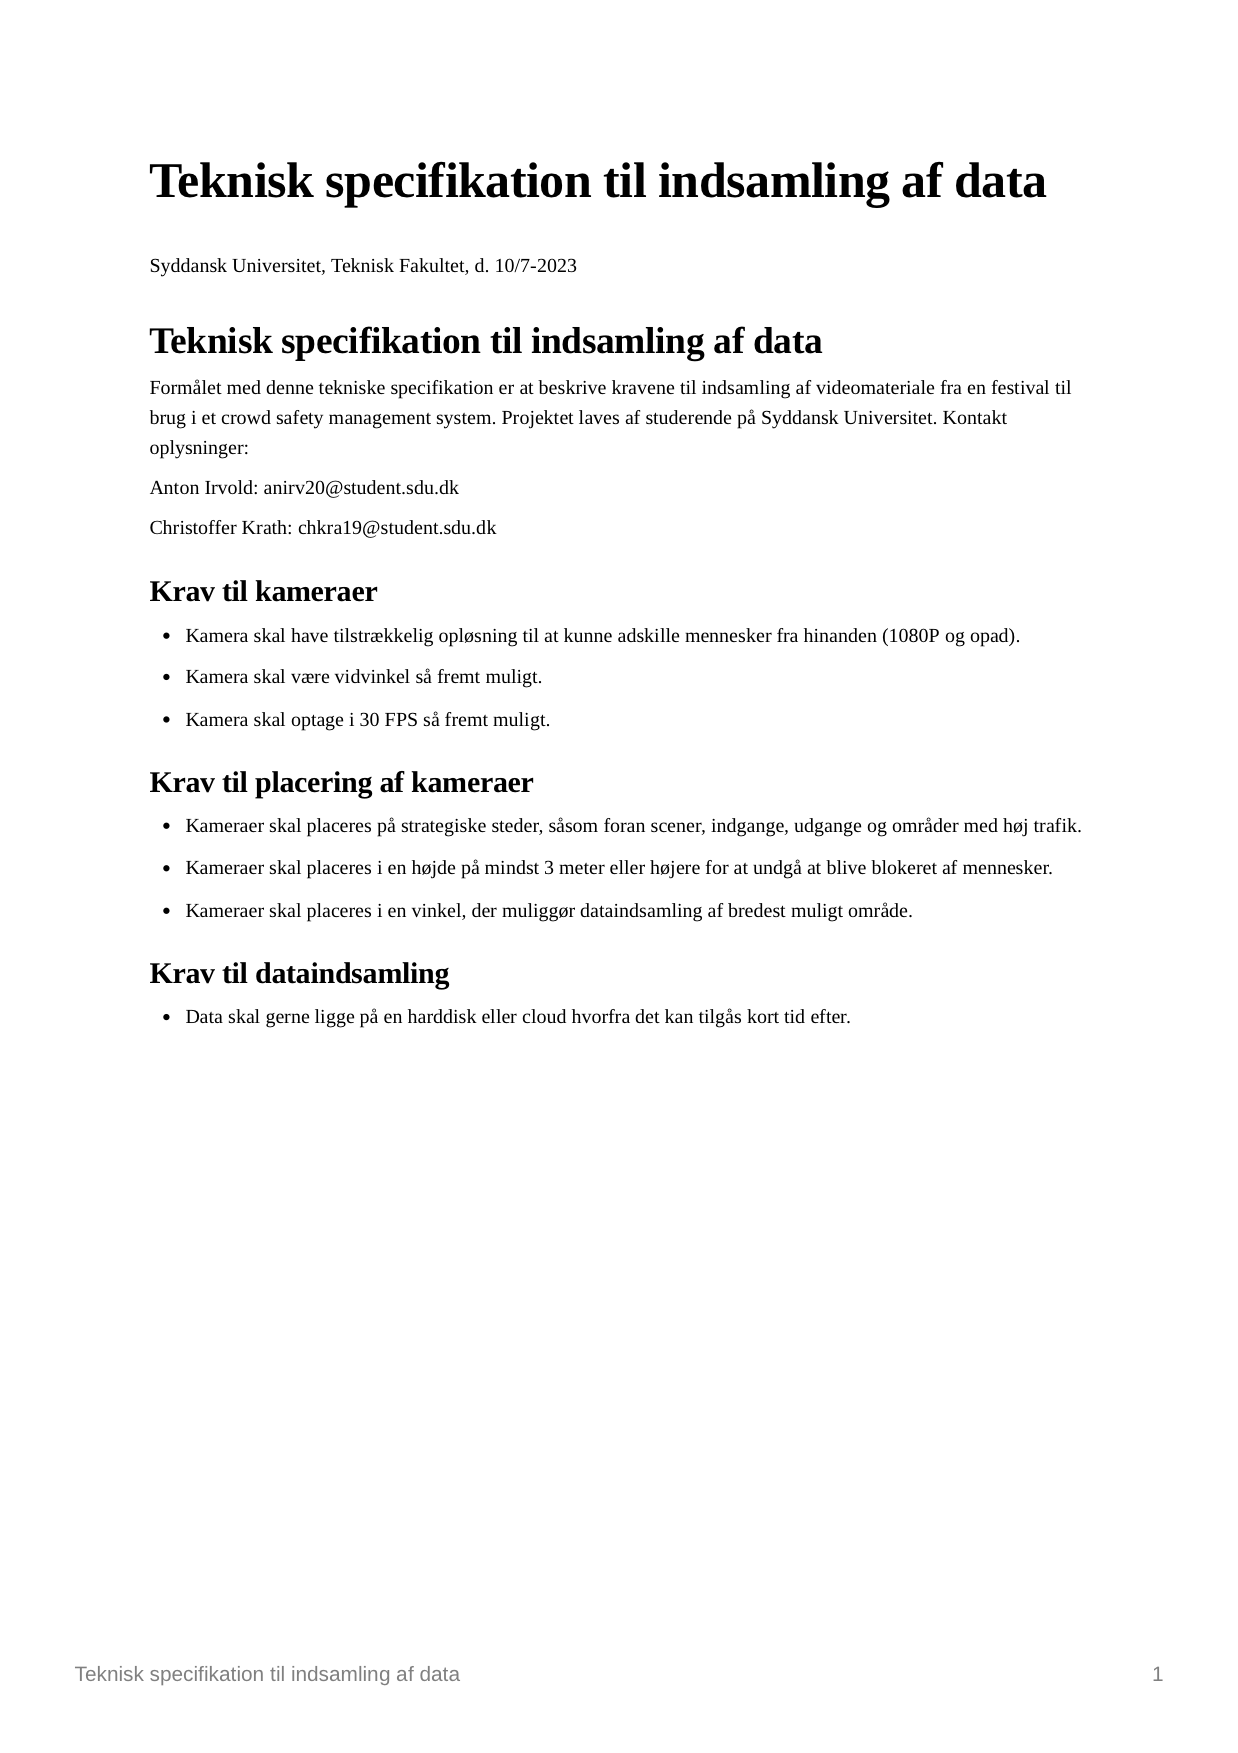
\includegraphics[width=1\textwidth,height=1\textheight]{../appendices/teknisk-specifikation.png}

\hypertarget{timeline}{%
\subsection{Timeline}\label{timeline}}

\begin{longtable}[]{@{}
  >{\raggedright\arraybackslash}p{(\columnwidth - 2\tabcolsep) * \real{0.5000}}
  >{\raggedright\arraybackslash}p{(\columnwidth - 2\tabcolsep) * \real{0.5000}}@{}}
\toprule\noalign{}
\begin{minipage}[b]{\linewidth}\raggedright
\textbf{Date}
\end{minipage} & \begin{minipage}[b]{\linewidth}\raggedright
\textbf{Activity}
\end{minipage} \\
\midrule\noalign{}
\endhead
\bottomrule\noalign{}
\endlastfoot
July-August & Gathering data at attended festivals in collaboration with
Event Safety \\
& \\
August & Drafting the project description \\
& \\
31-08-2023 & Delivering the project description \\
& \\
09-09-2023 & Final discussion with Event Safety regarding the proposed
solutions, requirements and the project going forward \\
September & In-depth analysis of use cases (with Event Safety) In-depth
analysis of required technologies and methods used in academic
literature. Design of the system \\
& \\
25-09-2023 & Progress update with Event Safety regarding the design of
the system \\
& \\
October & Implementation of proof of concept system (primarily
backend) \\
& \\
26-10-2023 & Progress update with Event Safety and small-scale user
testing \\
& \\
31-10-2023 & Attending Crowd Safety Course hosted by Event Safety in
Copenhagen \\
& \\
November & Implementation of proof of concept system \\
& \\
December & Final implementation of the system Documentation of the
system User testing and evaluation \\
\end{longtable}

\begin{quote}
\begin{quote}
\begin{quote}
\begin{quote}
\begin{quote}
\begin{quote}
\begin{quote}
877dd9d (updates quarto template)
\end{quote}
\end{quote}
\end{quote}
\end{quote}
\end{quote}
\end{quote}
\end{quote}


\printbibliography[title=References]


\end{document}
